\documentclass[10pt, aspectratio=1610]{beamer}

\usetheme{default} % theme général du diaporama

% Remove navigation icons
\beamertemplatenavigationsymbolsempty

% paquets pour le français
\usepackage[T1]{fontenc}
\usepackage[utf8]{inputenc}
% For figure manipulations
\usepackage{graphicx}
% Use quotes
\usepackage{csquotes}
% Equalize table columns widths
\usepackage{tabularx}
% Use tables larger than textwidth
\usepackage{adjustbox}

% Set height of table rows relative to maximum
\renewcommand{\arraystretch}{1.25}

% Bottom align tabularx headers
\renewcommand{\tabularxcolumn}[1]{b{#1}}

% Number figures
\setbeamertemplate{caption}[numbered]

% use serif font with rm
% \renewcommand{\familydefault}{\rmdefault}

\title{Spatially continuous identification of beta diversity hotspots using species distribution models}
\author{
  Gabriel Dansereau\inst{1,2,3}
  \and
  Timothée Poisot\inst{1,2,3,4}
  \and
  Pierre Legendre\inst{1,3}
}
\institute{
  \inst{1} Département de sciences biologiques, Université de Montréal
  \and
  \inst{2} BIOS\textsuperscript{2}
  \and
  \inst{3} Quebec Center for Biodiversity Science
  \and
  \inst{4} Groupe de recherche interuniversitaire en limnologie et environnement aquatique
}
\date{
  10th Annual QCBS Symposium\\
  December 19, 2019
}
% Affiliation logos
\titlegraphic{
  \hspace{1cm} 
\includegraphics[scale=0.05]{fig/logo-udem.png}\hfill
  
\includegraphics[scale=0.4]{fig/logo-bios2}\hfill
  
\includegraphics[scale=0.25]{fig/logo-csbq.png}\hfill
  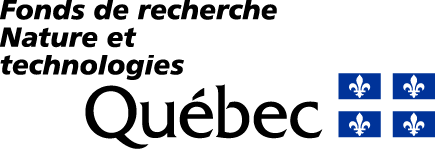
\includegraphics[scale=0.5]{fig/logo-frqnt.png}\hspace{1cm}
}
% Bird logo
\logo{%
   
\includegraphics[scale=0.05]{fig/logo-warbler2.png}\hspace*{0.84\paperwidth}~%
   
\includegraphics[scale=.075]{fig/logo-bird.png}
}

\begin{document}

\begin{frame}
  \titlepage
\end{frame}

\begin{frame}
  \frametitle{Suggestion}
  \vspace*{0.5cm}
  Bring together 2 elements:
  \begin{enumerate}
    \item Identification of beta diversity hotspots
    \item Species distribution modelling (SDM) on continuous scales
  \end{enumerate}
  \begin{figure}
    \centering
    \hspace*{0.0cm}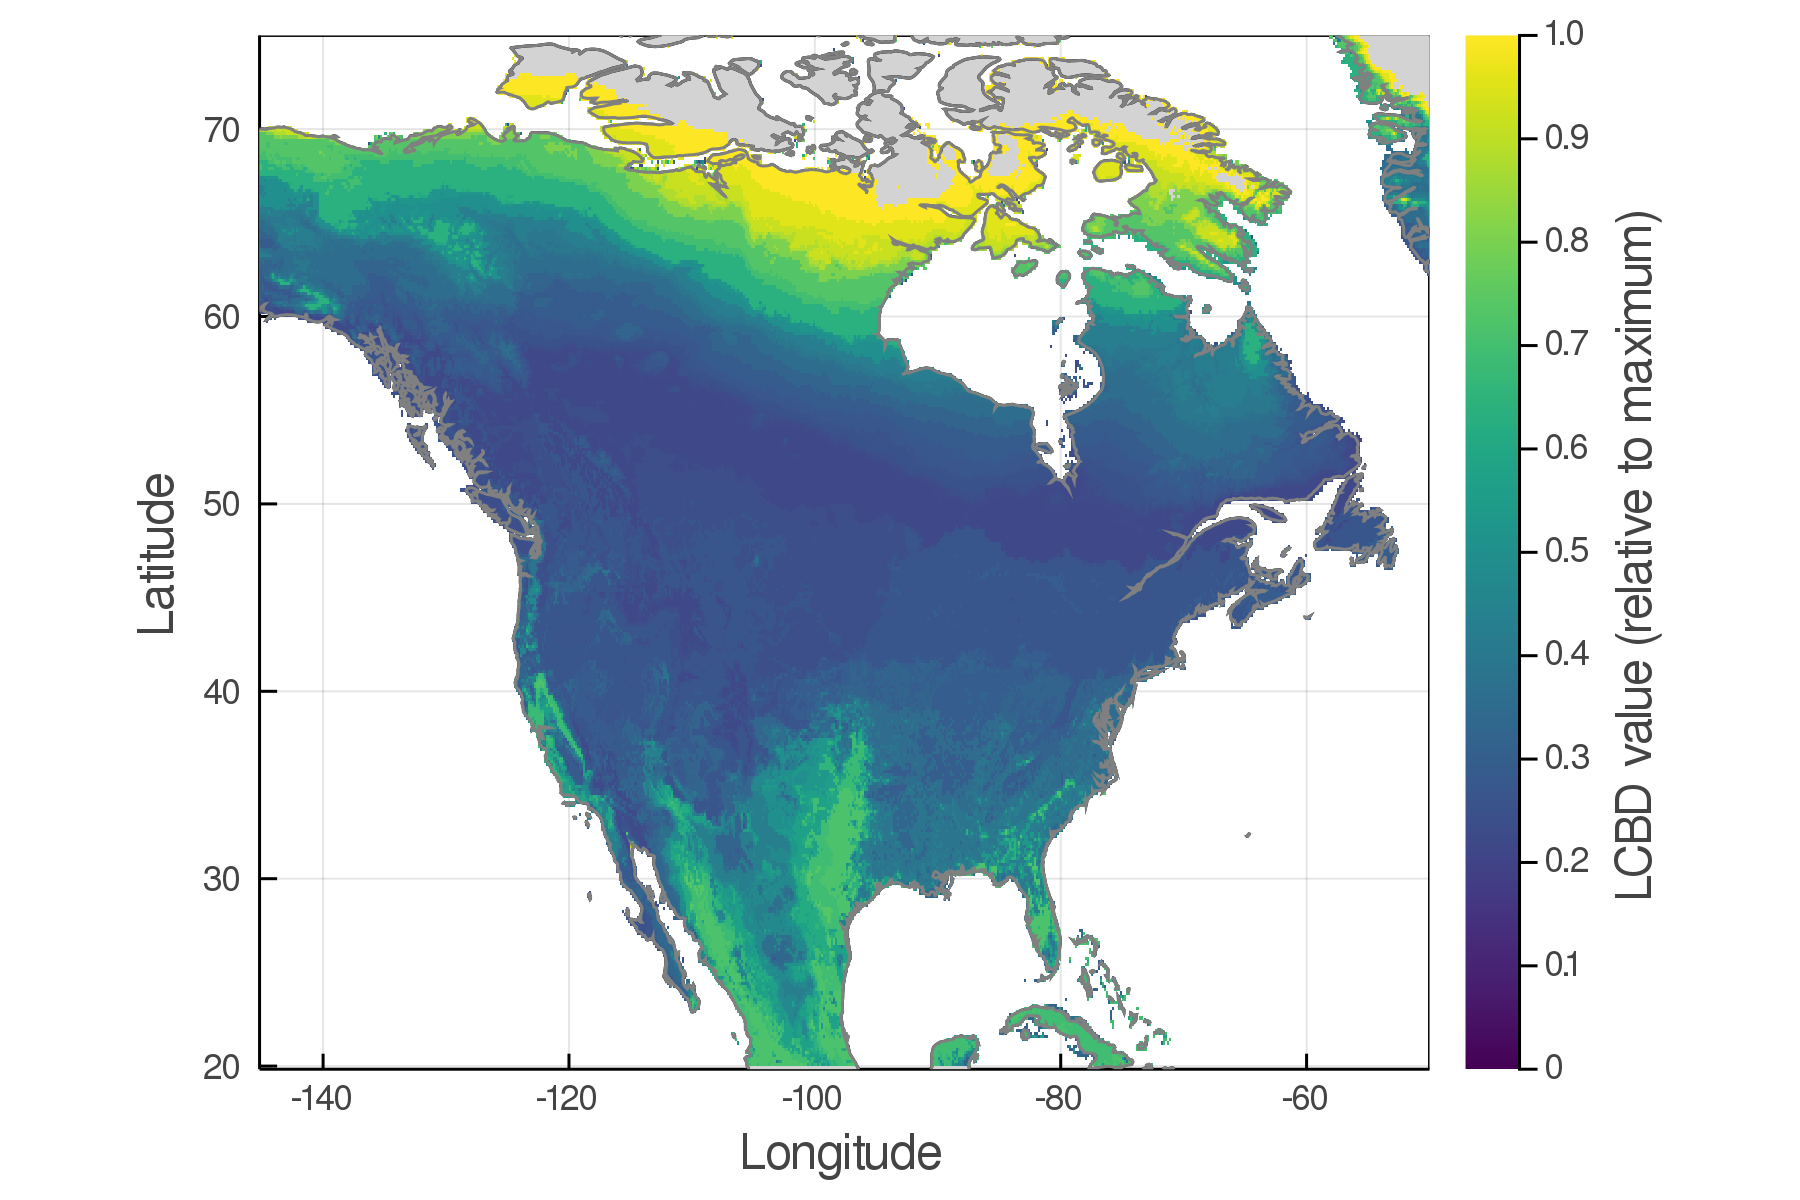
\includegraphics[scale=0.15]{fig/05_sdm_lcbd.png}
  \end{figure}
\end{frame}

\begin{frame}
  \frametitle{While we're at it...}
  Beta diversity
  \begin{itemize}
    \item Community composition, not turnover
  \end{itemize}
  \medskip
  \begin{quotation}
    "Variation in species composition among sites within a geographical region of interest" (Legendre et al. 2005)
  \end{quotation}
  \vfill
  Local contribution to beta diversity (LCBD)
  \begin{itemize}
    \item Highlights exceptional species compositions
  \end{itemize}
  \medskip
  \begin{quotation}
    "Comparative indicators of the ecological uniqueness of sites in terms of community composition" (Legendre \& De Caceres, 2013)
  \end{quotation}
  \vfill
\end{frame}

\begin{frame}
  \frametitle{Why continuous scales?}
  \begin{figure}
    \centering
    \hspace*{-0cm}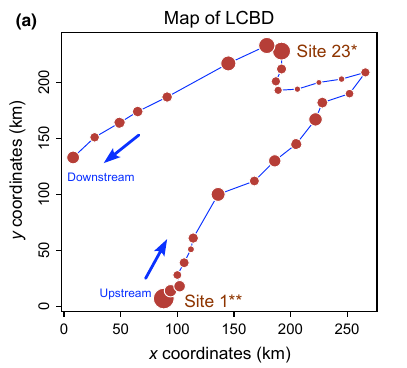
\includegraphics[scale=0.5]{fig/lcbd_LegeDeCa2013.png}
  \end{figure}
  \centering
  Original LCBD example (Legendre \& De Caceres, 2013)
\end{frame}

\begin{frame}
  \frametitle{Why continuous scales?}
  \begin{itemize}
    \item Online data on extended scales is increasingly accessible
    \item Potential for novel ecological insights
  \end{itemize}
  \begin{figure}
    \centering
    \hspace*{-1cm}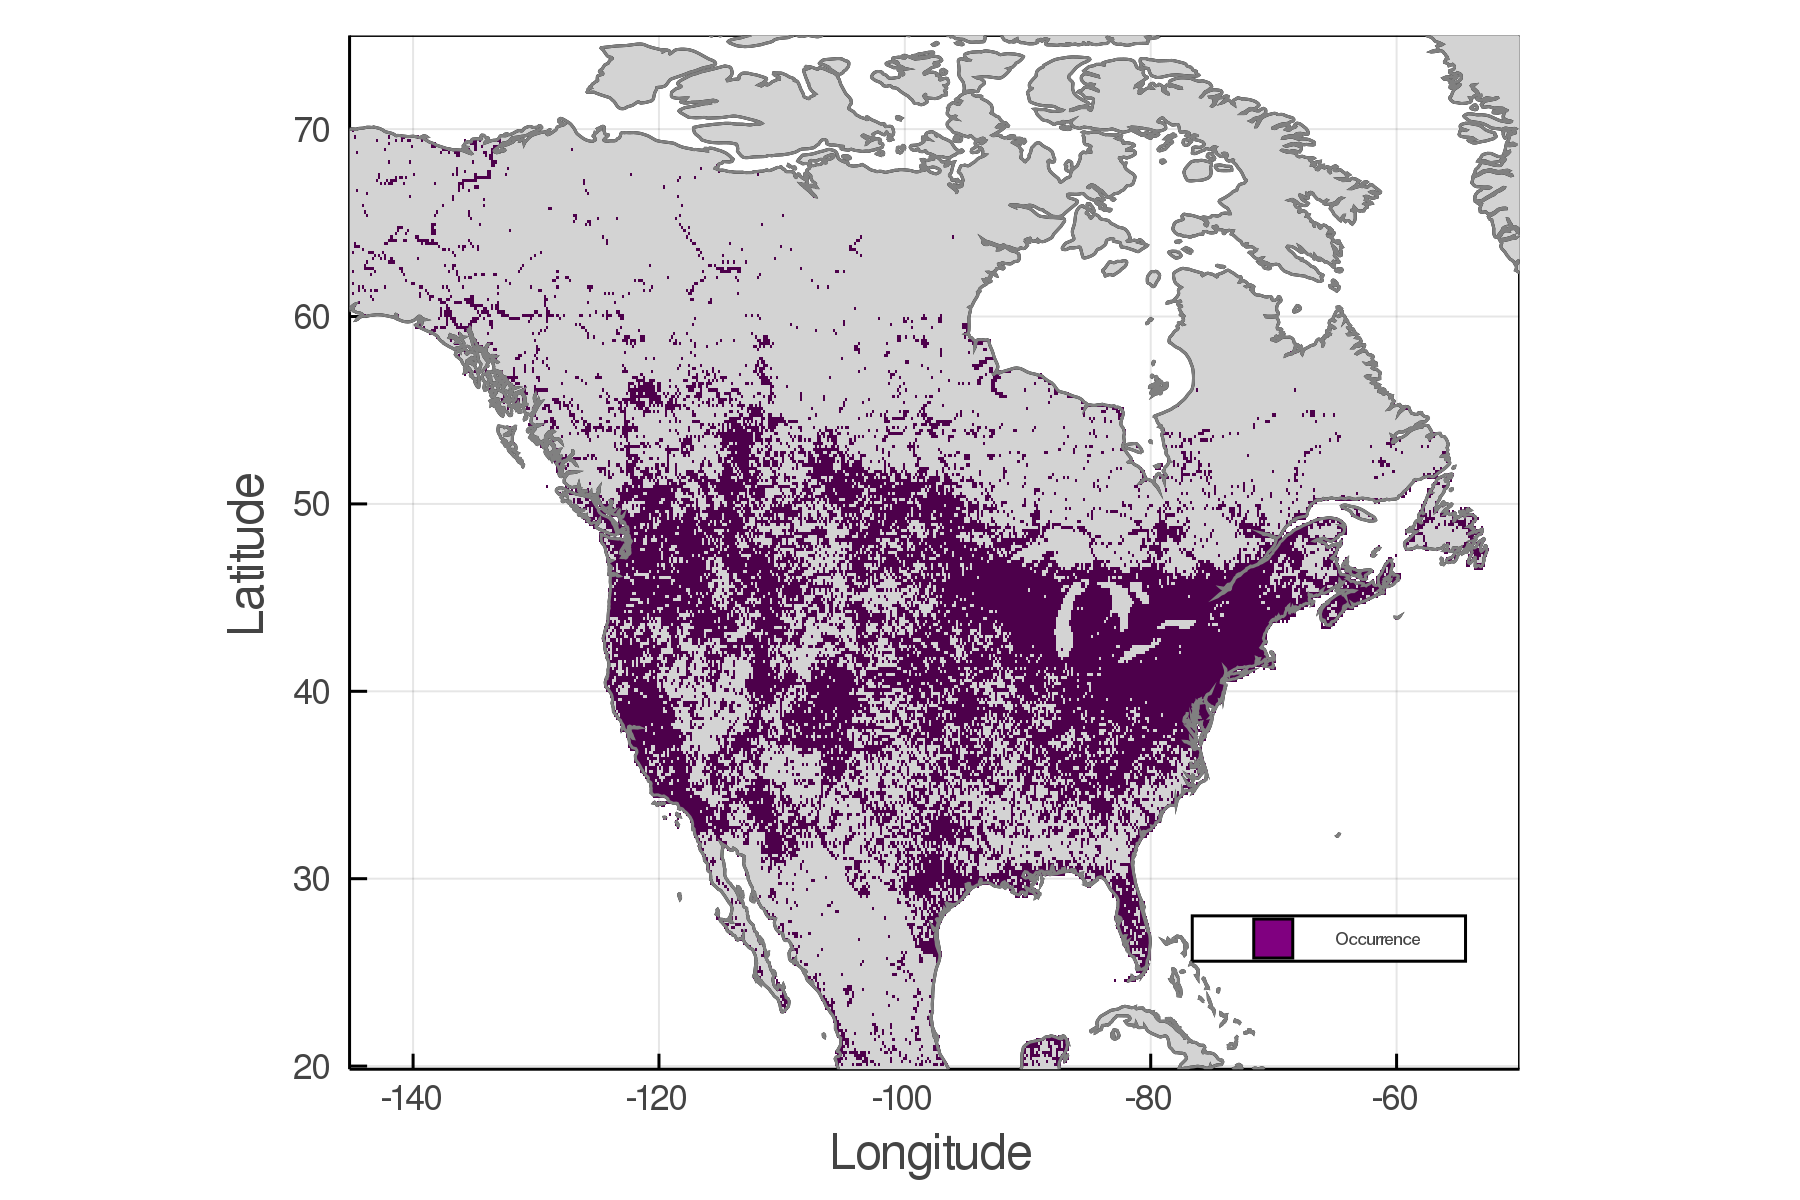
\includegraphics[scale=0.12]{fig/01_raw_singlesp.png}%
    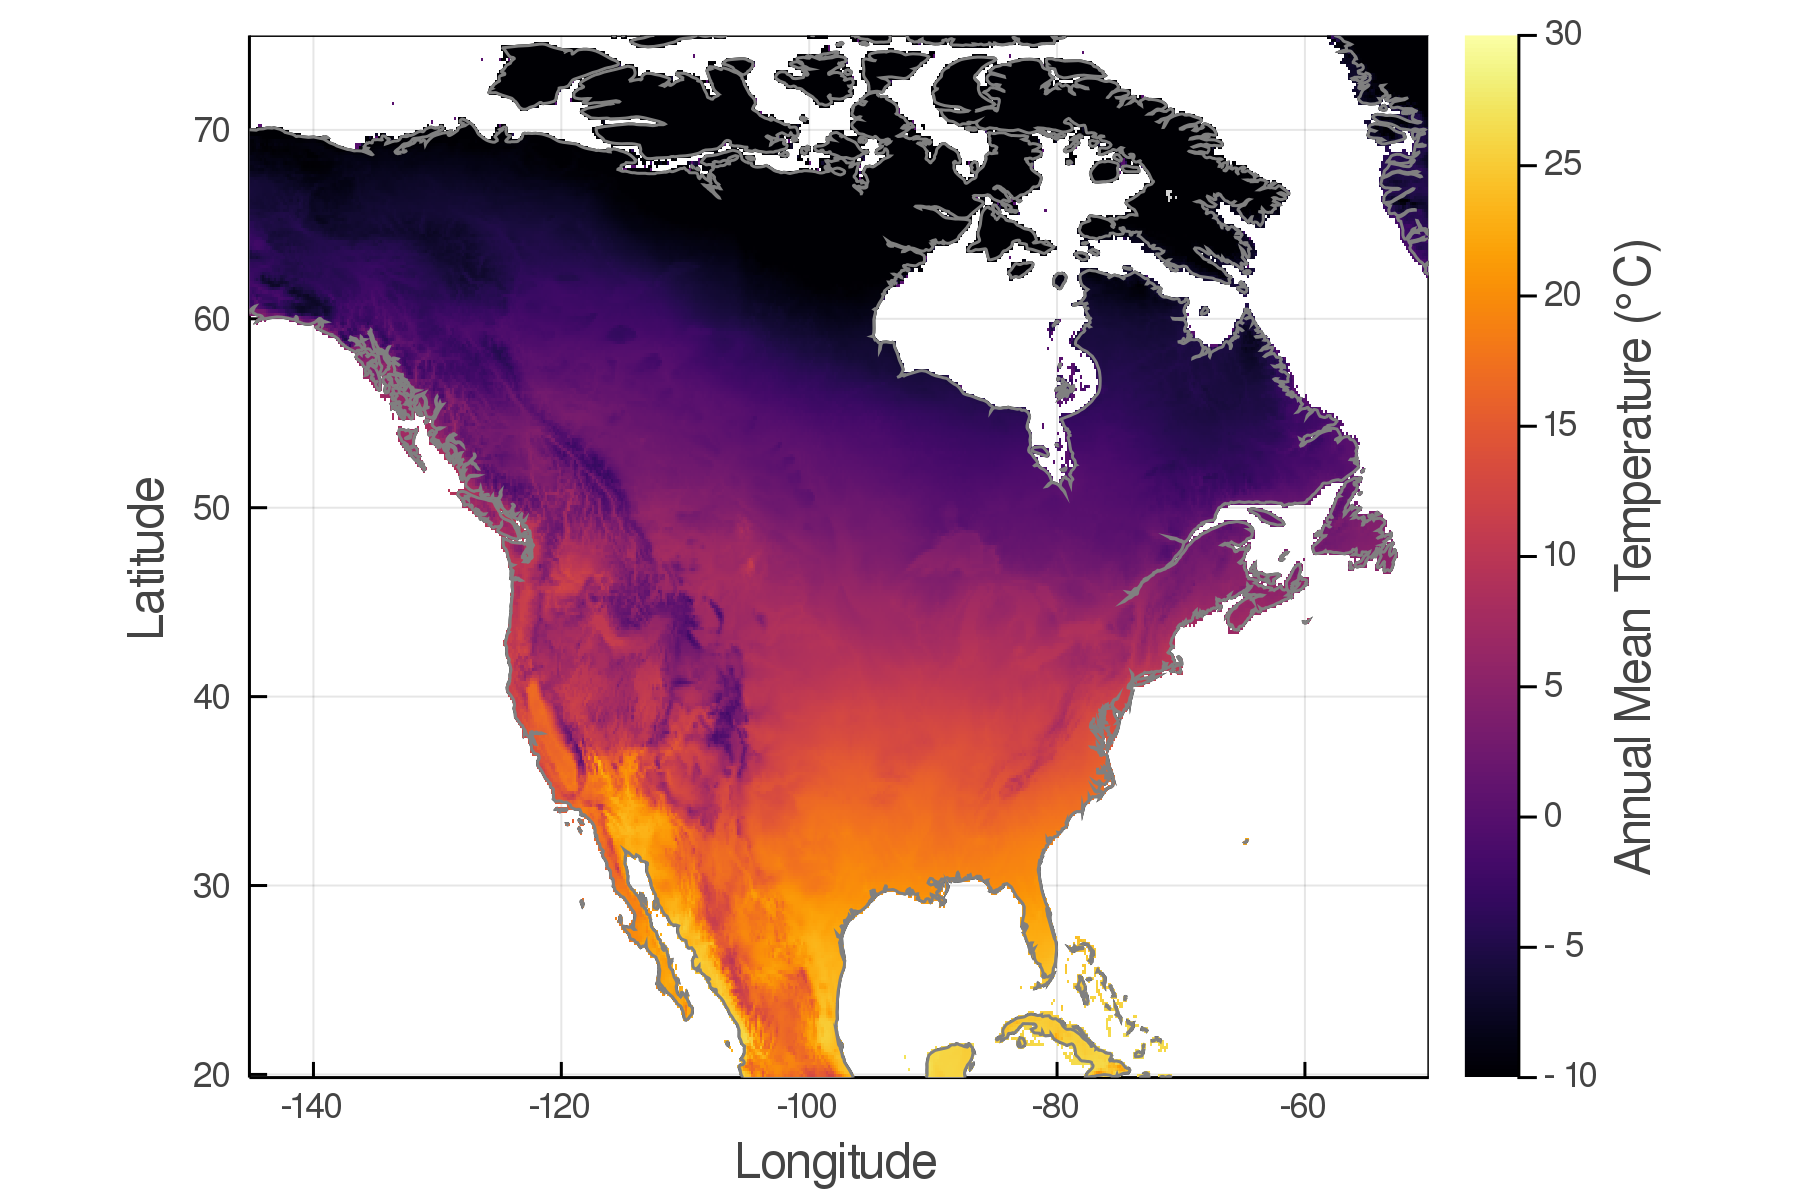
\includegraphics[scale=0.12]{fig/wc_temp.png}
  \end{figure}
\end{frame}

\begin{frame}
  \frametitle{Relevance}
  \begin{columns}
    \hspace*{-0cm}\column{0.6\textwidth}
      Novel ecological insights
      \begin{itemize}
        \item Tool for poorly sampled regions, or with sparse sampling
        \item Identification of conservation targets
      \end{itemize}
      \vspace{0.5cm}
      Combination with IPCC climate change scenarios
      \begin{itemize}
        \item Model beta diversity changes
        \item Identify sites with significant changes
      \end{itemize}
      \vspace{0.5cm}
      $\Rightarrow$ Insight-oriented approach, exploratory analyses
    \hspace*{-1cm}\column{0.5\textwidth}
      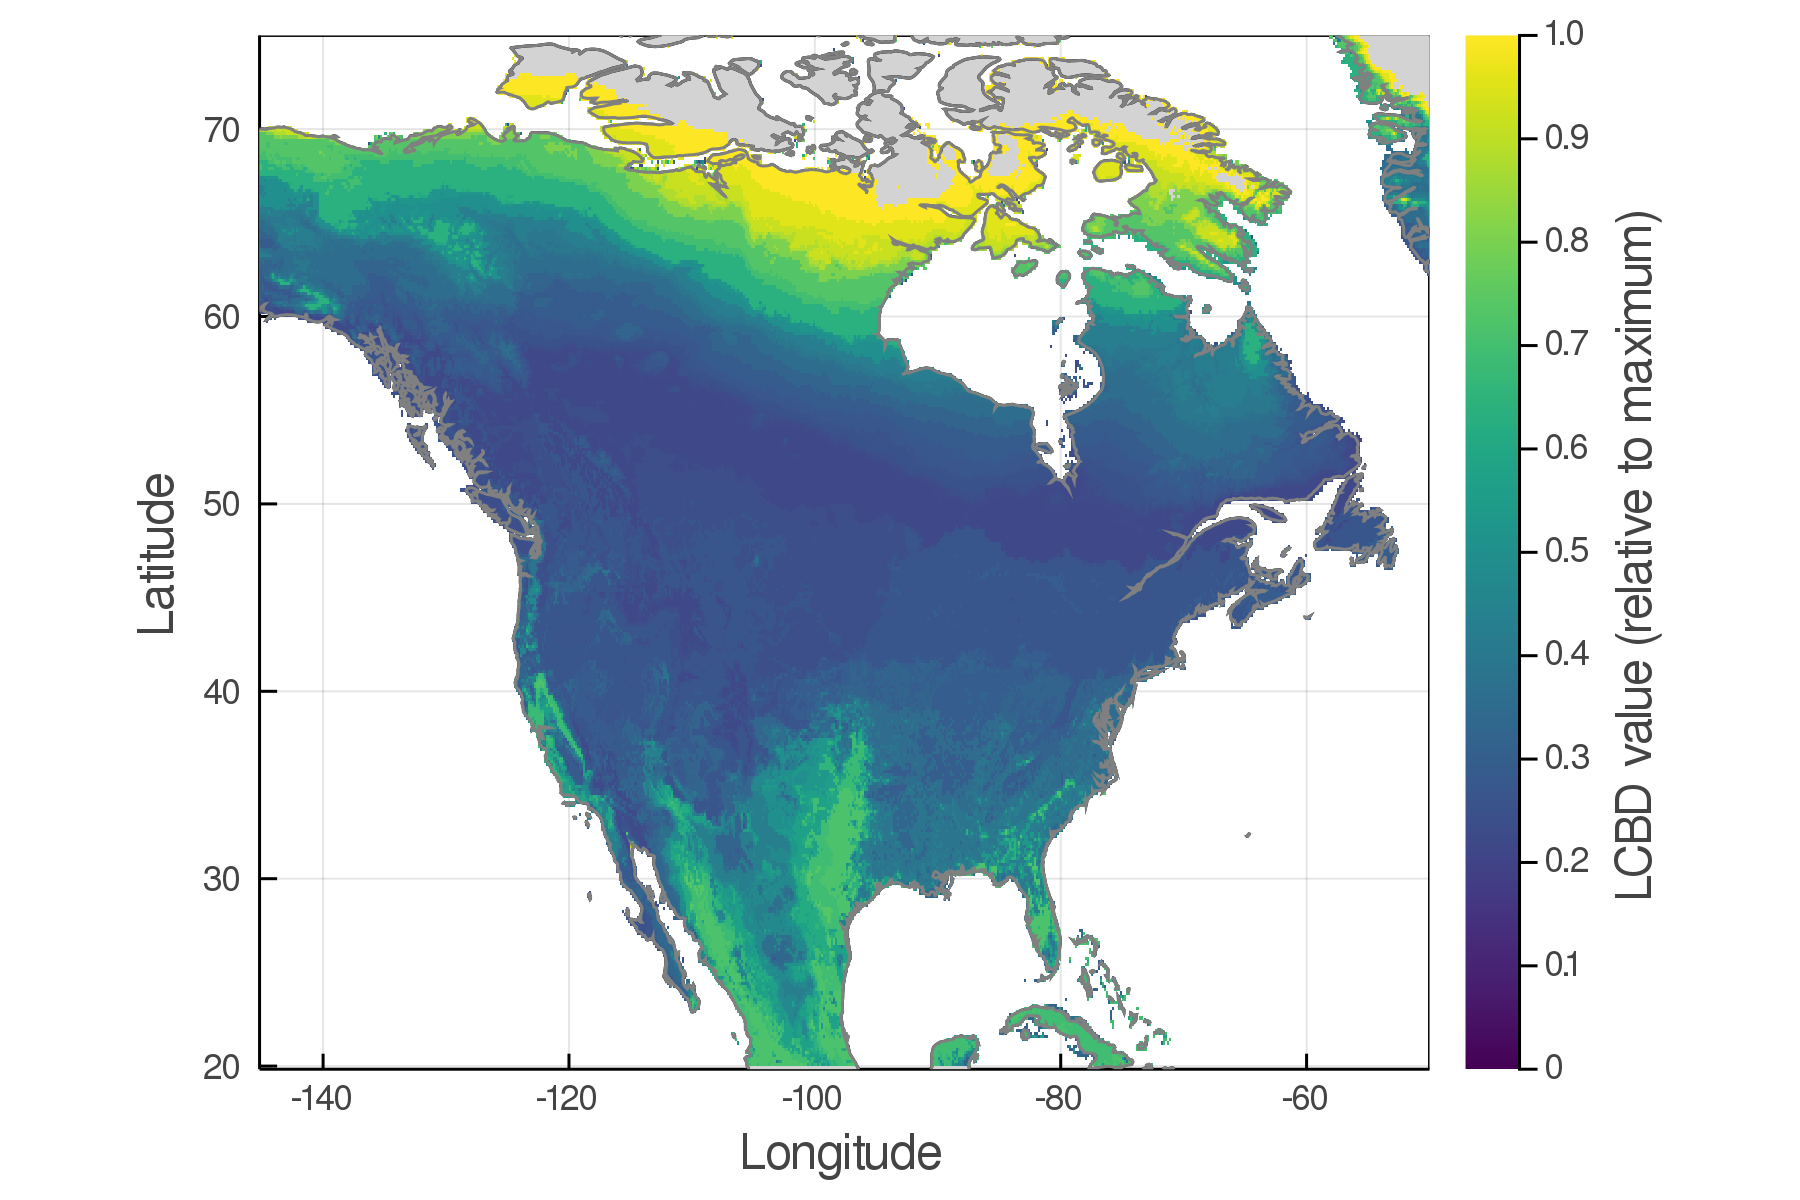
\includegraphics[scale=0.12]{fig/05_sdm_lcbd.png}
  \end{columns}
\end{frame}

\begin{frame}
  \frametitle{Occurrence data}
  \hspace*{0.5cm}
  \begin{itemize}
    \item Data from the eBird Basic Dataset
    \item All species of Warblers (\textit{Parulidae} family) in North America
  \end{itemize}
  \begin{figure}
    \centering
    \hspace*{-1cm}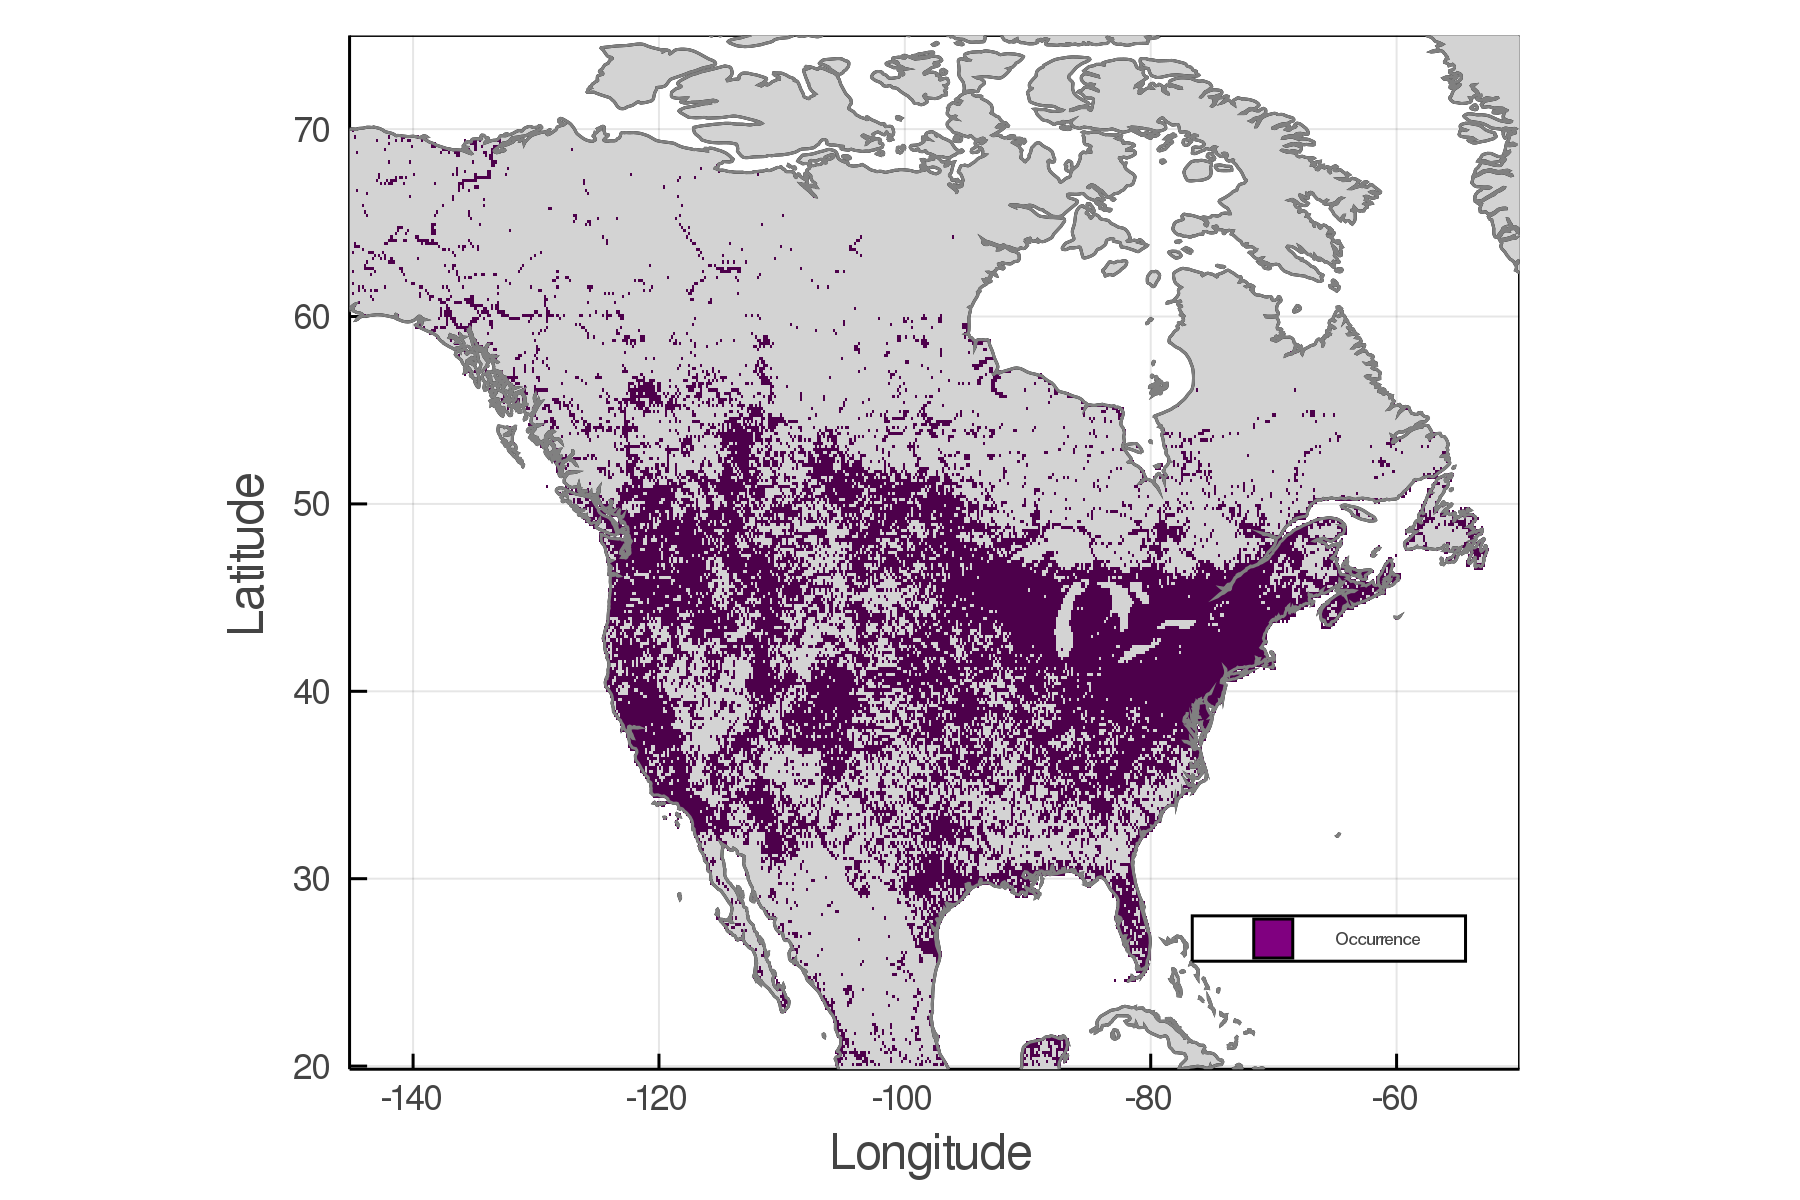
\includegraphics[scale=0.135]{fig/01_raw_singlesp.png}%
    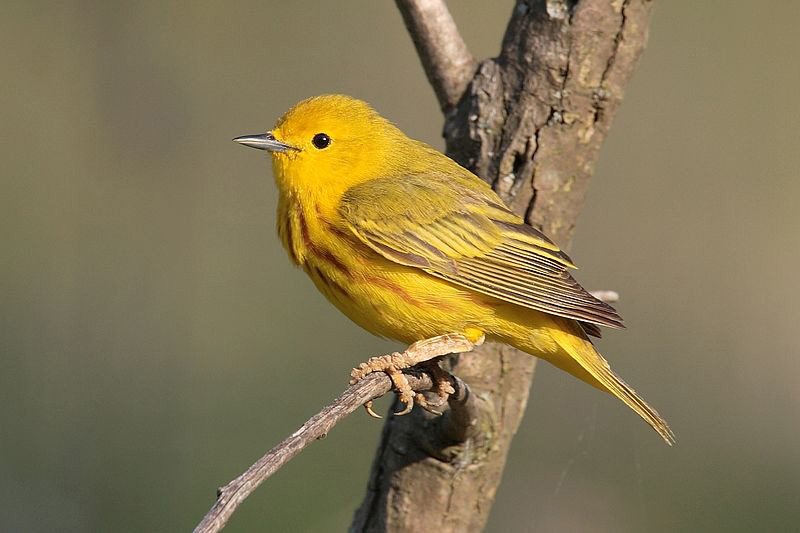
\includegraphics[scale=0.60]{fig/yellow-warbler.jpg}
    
\includegraphics[scale=1.3]{fig/logo-ebird.png}
  \end{figure}
\end{frame}

\begin{frame}
  \frametitle{Environmental data}
  \hspace*{0.5cm}
  \begin{itemize}
    \item 2 climates variables : mean annual temperature, mean annual precipitation
    \item 10 land cover variables : bare, crops, grass, moss, shrub, snow, tree, urban, permanent water, seasonal water
  \end{itemize}
  \begin{figure}
    \centering
    \hspace*{-0.5cm}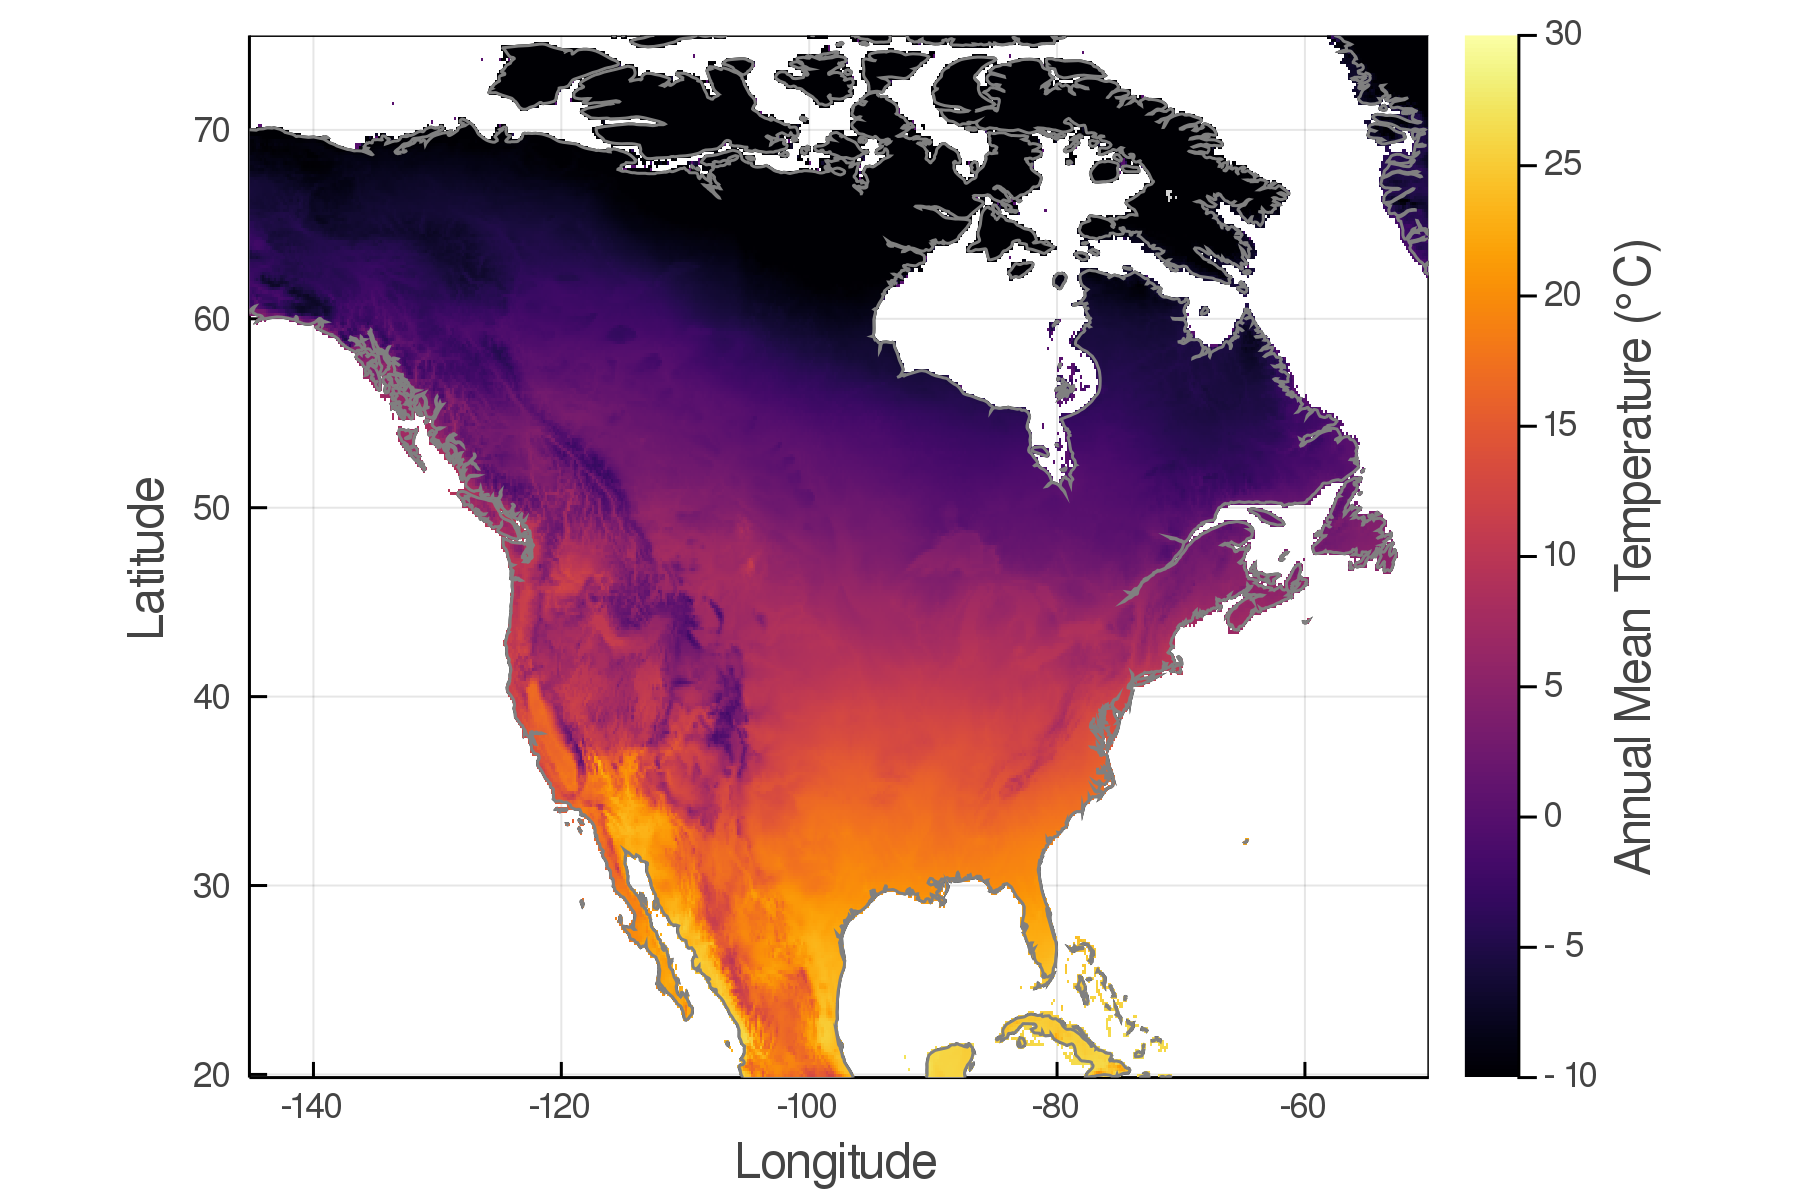
\includegraphics[scale=0.12]{fig/wc_temp.png}%
    \hspace*{0.5cm}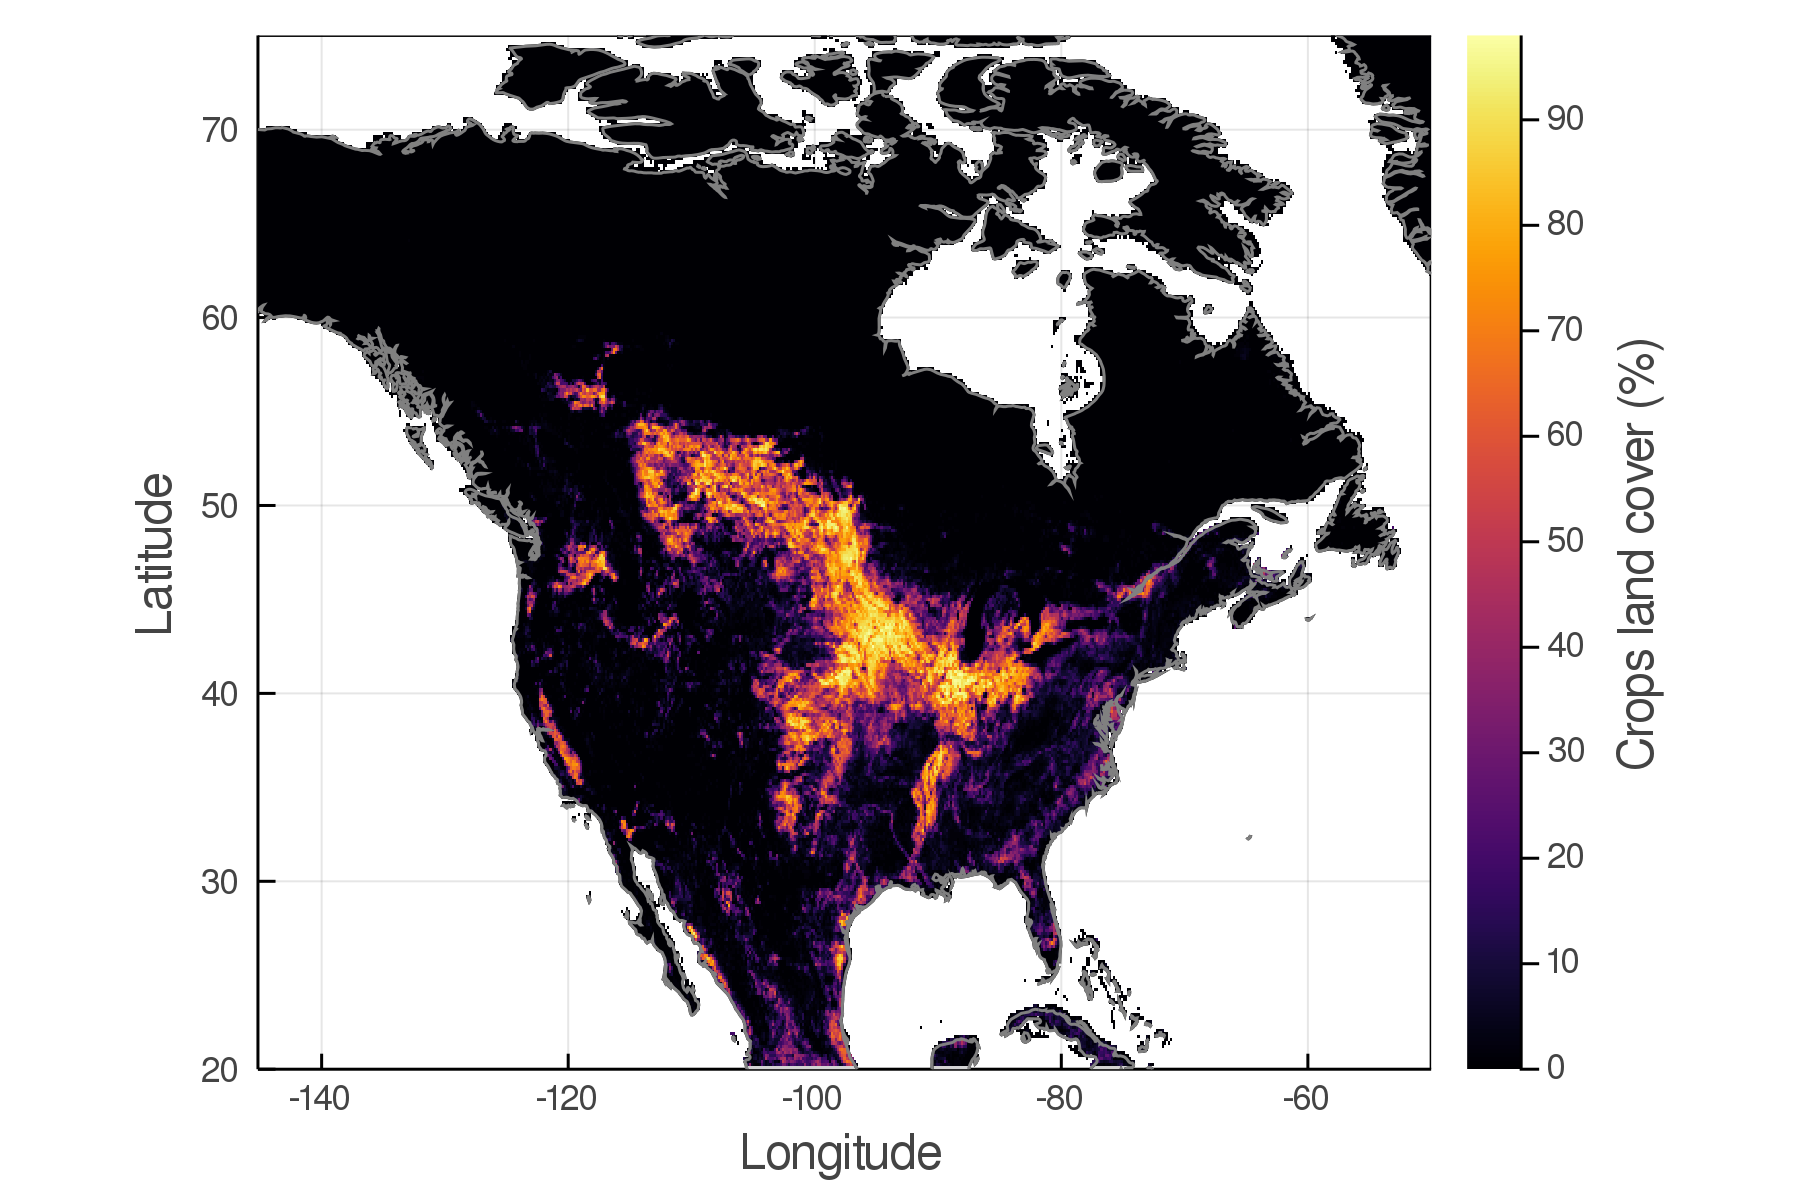
\includegraphics[scale=0.12]{fig/lc_temp.png}
  \end{figure}
  \begin{figure}
    \centering
    \hspace*{-1cm}
\includegraphics[scale=0.20]{fig/logo-worldclim.png}%
    \hspace*{4.5cm}
\includegraphics[scale=0.40]{fig/logo-copernicus.png}
  \end{figure}
\end{frame}

\begin{frame}
  \frametitle{Methods - BIOCLIM model}
  \begin{figure}
    \centering
    \hspace*{-0cm}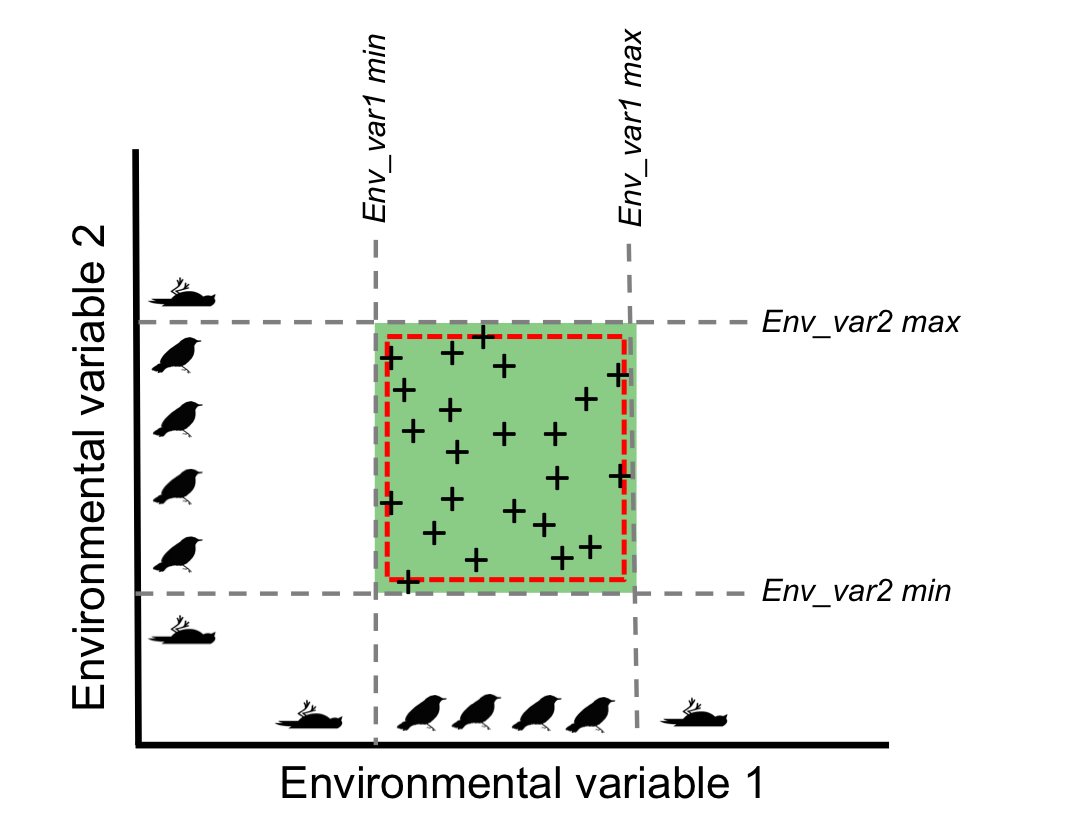
\includegraphics[scale=0.25]{fig/bioclim_bccvl.png}
  \end{figure}
  \centering
  Climate envelope in the BIOCLIM model\footnote{\tiny https://support.bccvl.org.au/support/solutions/articles/6000083201-bioclim}
\end{frame}

\begin{frame}
  \frametitle{Species richness - Raw data}
  \begin{figure}
    \centering
    \hspace*{-0cm}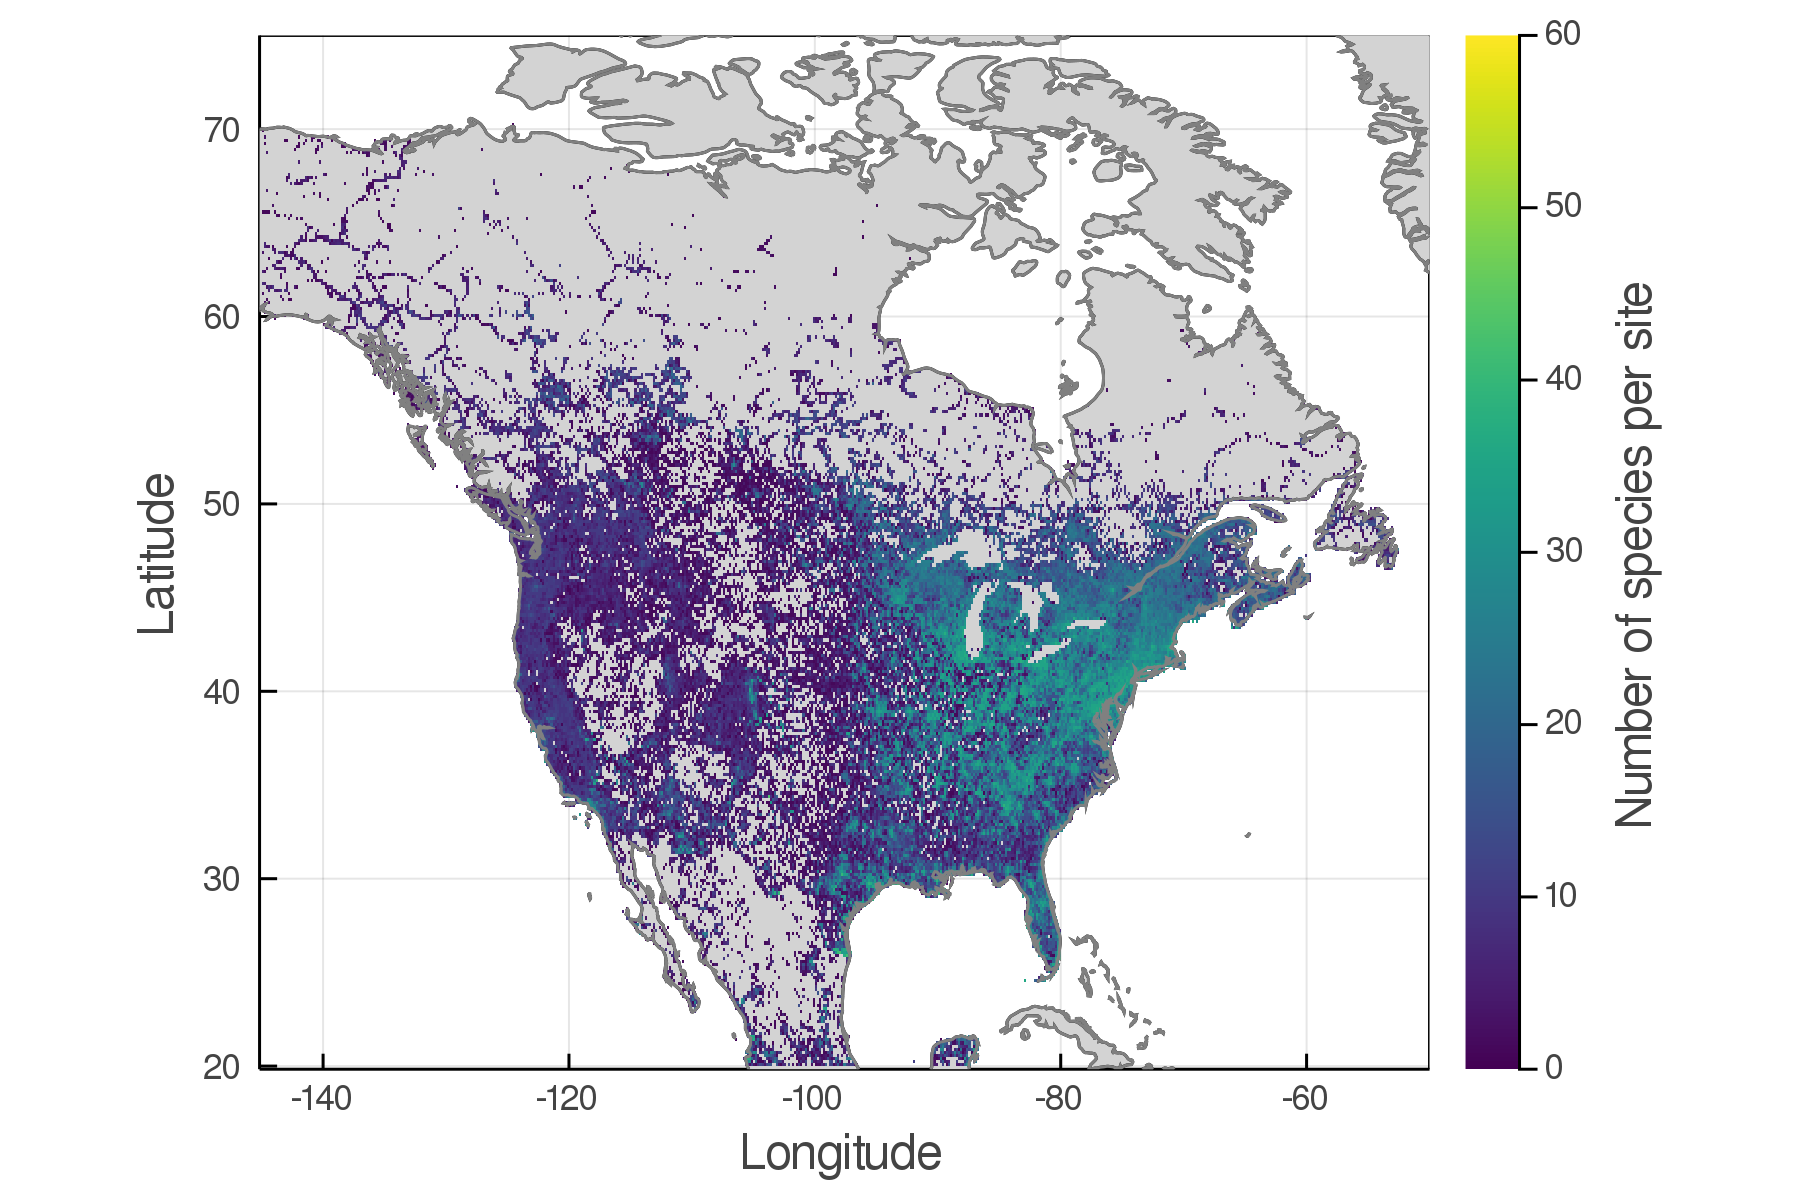
\includegraphics[scale=0.20]{fig/03_raw_richness.png}
  \end{figure}
\end{frame}

\begin{frame}
  \frametitle{Species richness - SDM results}
  \begin{figure}
    \centering
    \hspace*{-0cm}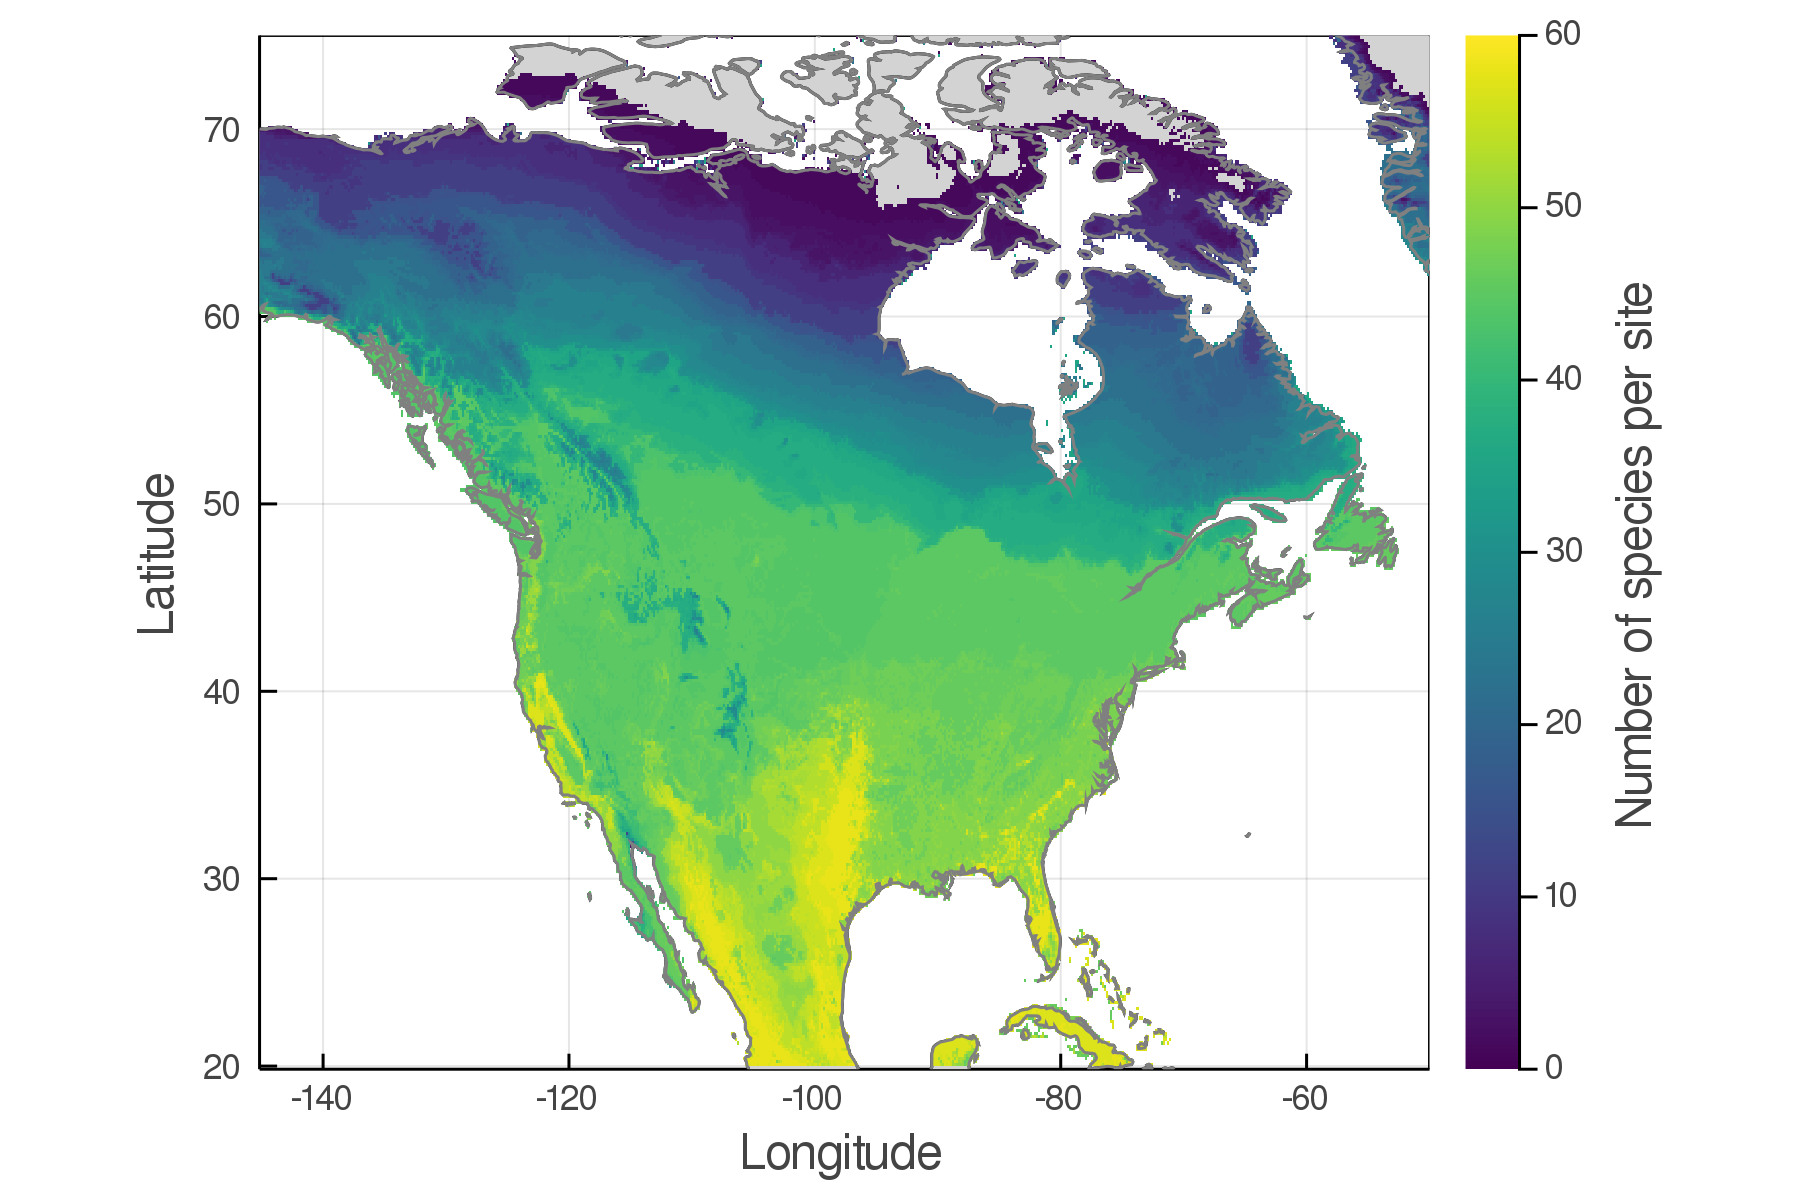
\includegraphics[scale=0.20]{fig/03_sdm_richness.png}
  \end{figure}
\end{frame}

\begin{frame}
  \frametitle{LCBD values - SDM results}
  \begin{figure}
    \centering
    \hspace*{-0cm}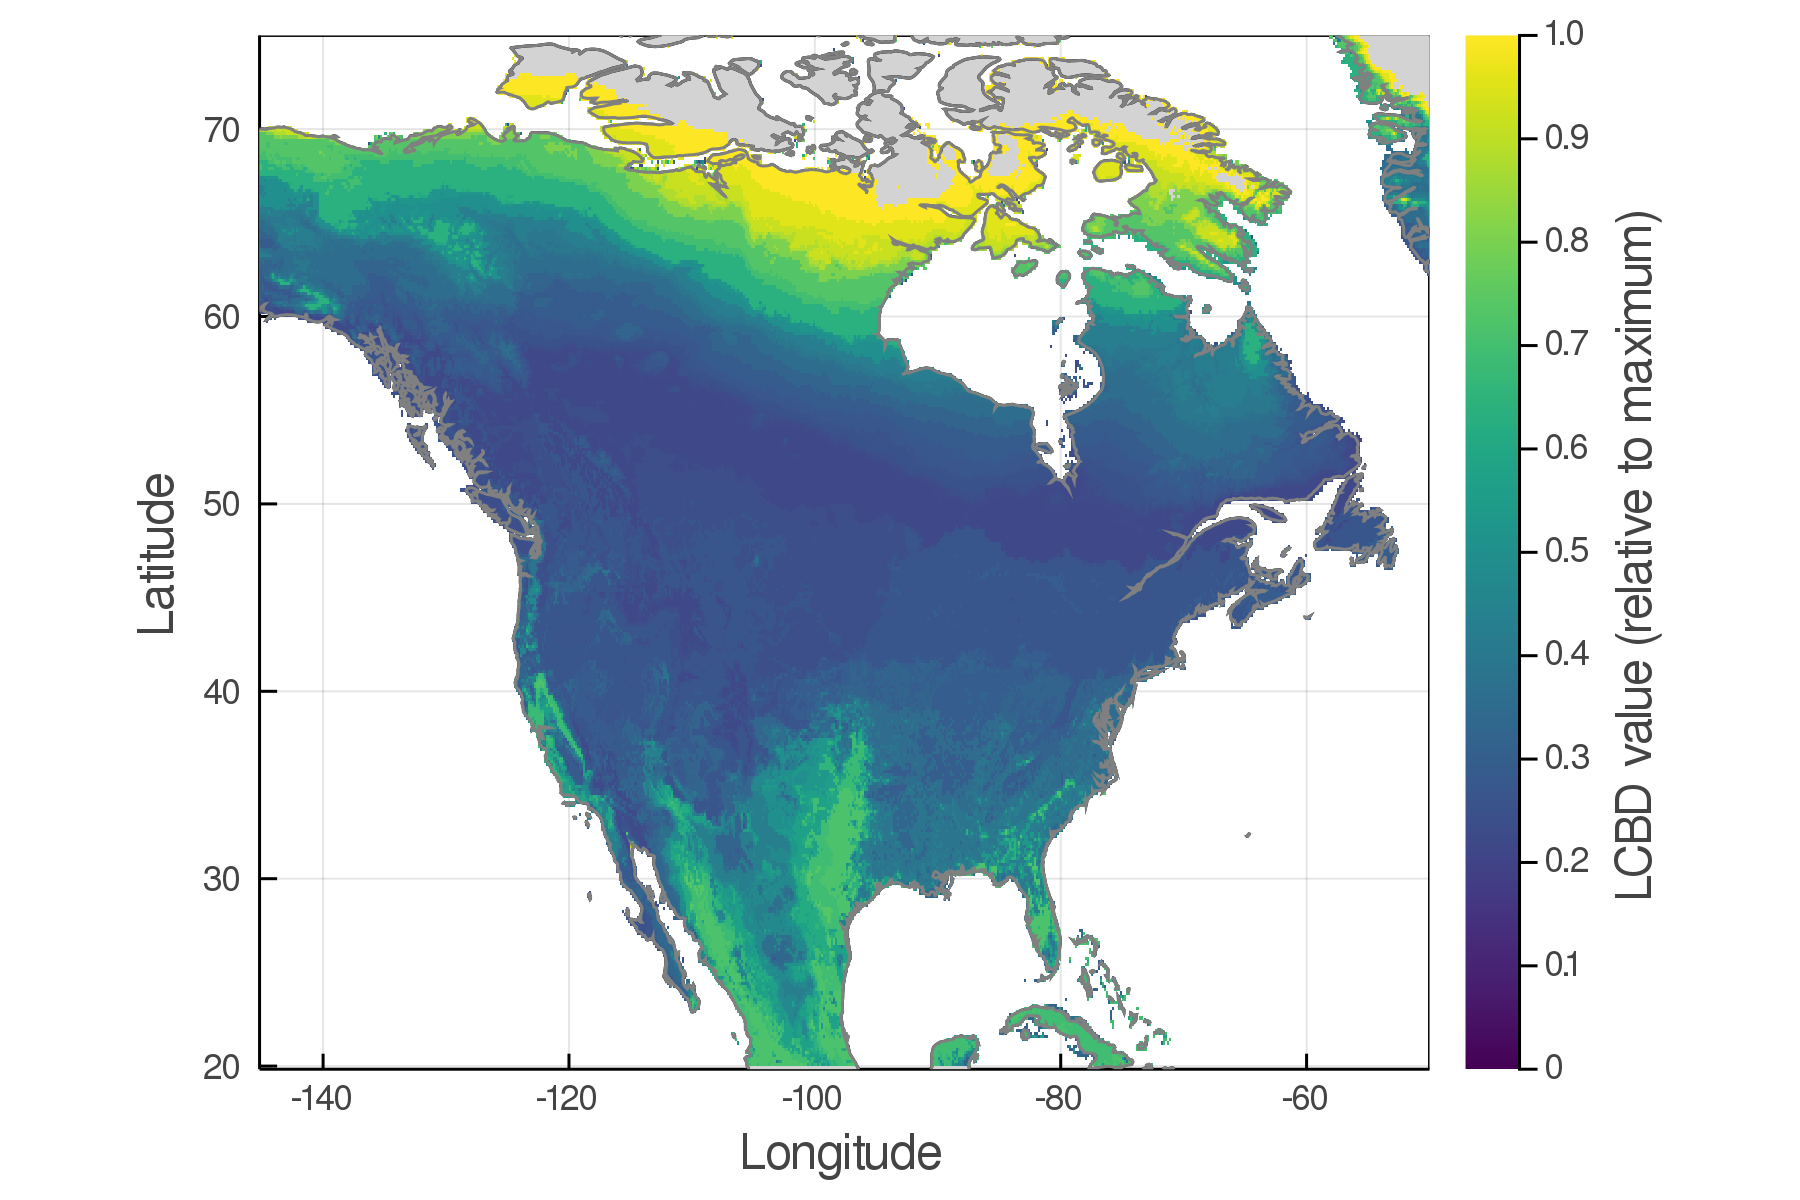
\includegraphics[scale=0.20]{fig/05_sdm_lcbd.png}
  \end{figure}
\end{frame}

\begin{frame}
  \frametitle{LCBD-richness relationship}
  \begin{figure}
    \centering
    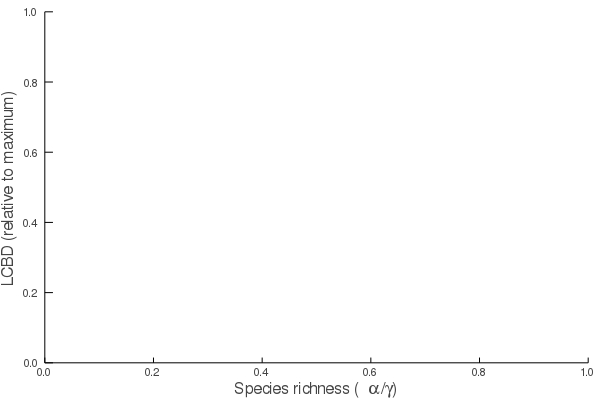
\includegraphics[scale=0.5]{fig/06_cmb_relation-oneplot-empty.png}
  \end{figure}
\end{frame}

\begin{frame}
  \frametitle{LCBD-richness relationship}
  \begin{figure}
    \centering
    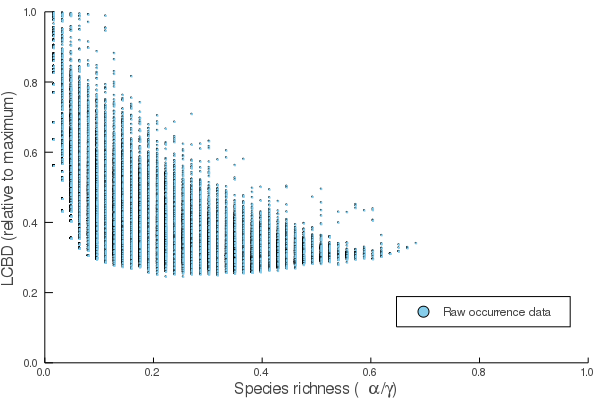
\includegraphics[scale=0.5]{fig/06_raw_relation.png}
  \end{figure}
\end{frame}

\begin{frame}
  \frametitle{LCBD-richness relationship}
  \begin{figure}
    \centering
    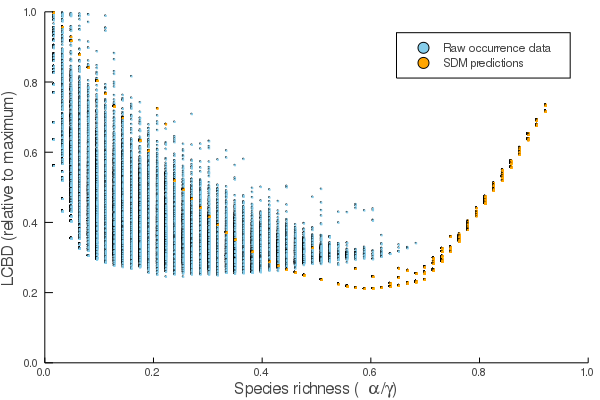
\includegraphics[scale=0.5]{fig/06_cmb_relation-oneplot.png}
  \end{figure}
\end{frame}

\begin{frame}
  \centering \frametitle{Spatially continuous identification of beta-diversity hotspots using species distribution modelling}
  \begin{figure}
    \centering
    \hspace*{-2cm}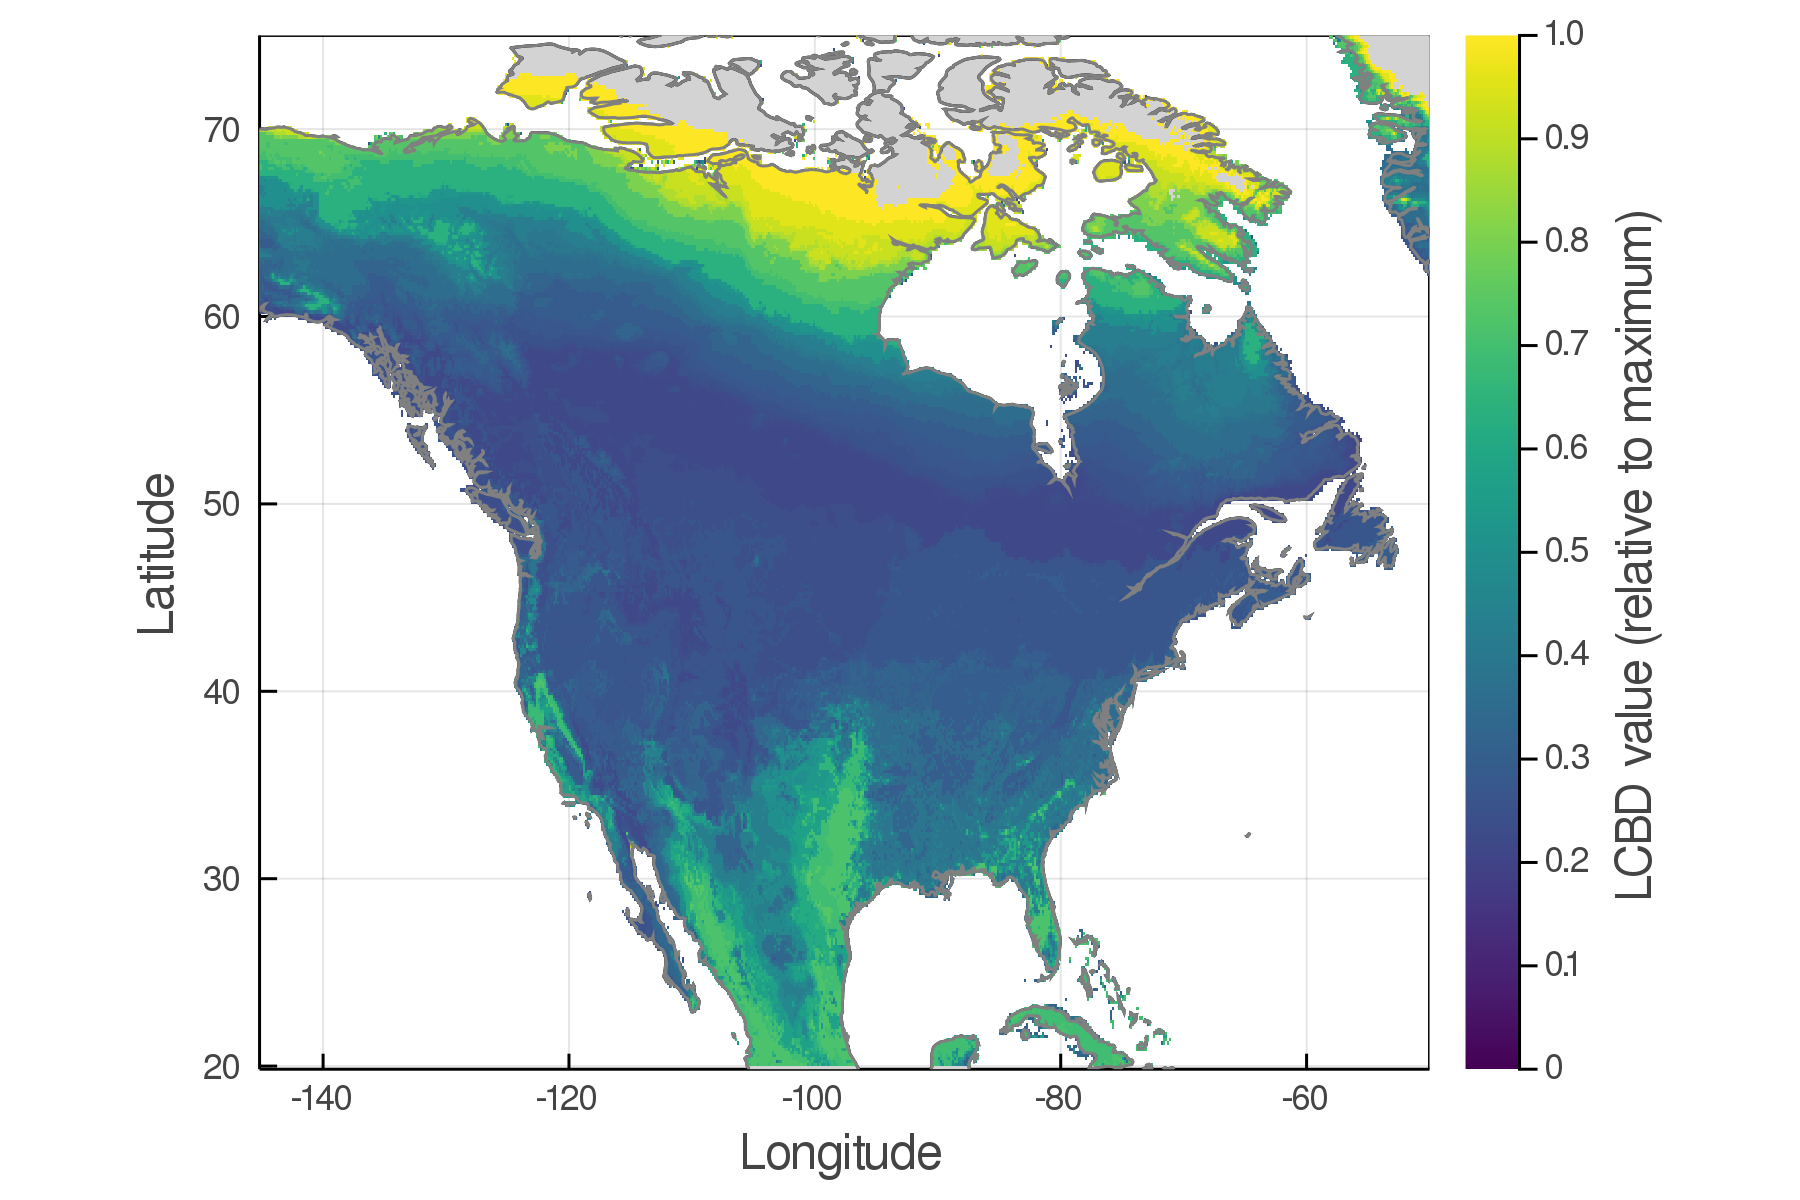
\includegraphics[scale=0.13]{fig/05_sdm_lcbd.png}
    \hspace*{-0cm}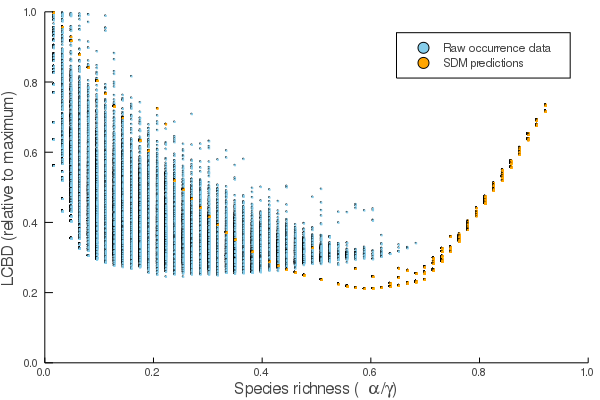
\includegraphics[scale=0.34]{fig/06_cmb_relation-oneplot.png}
  \end{figure}
  \medskip
  \centering
  Gabriel Dansereau

  gabriel.dansereau@umontreal.ca
\end{frame}

\begin{frame}
  \frametitle{Icon credits}
  \begin{figure}
    \centering
    \hspace*{-0cm}
\includegraphics[scale=0.15]{fig/logo-warbler2-cred.png}
    \hspace*{2cm}
\includegraphics[scale=0.20]{fig/logo-bird-cred.png}
  \end{figure}
\end{frame}

%%%%%%%%%%%%%%%%%%%%%%%%%%%%%%%%%%%%%%%%%%%%

\begin{frame}
  \vfill
  \centering
  \huge Appendix
  \vfill
\end{frame}

\begin{frame}
  \frametitle{Single species example - SDM with threshold}
  \begin{figure}
    \centering
    \hspace*{-0cm}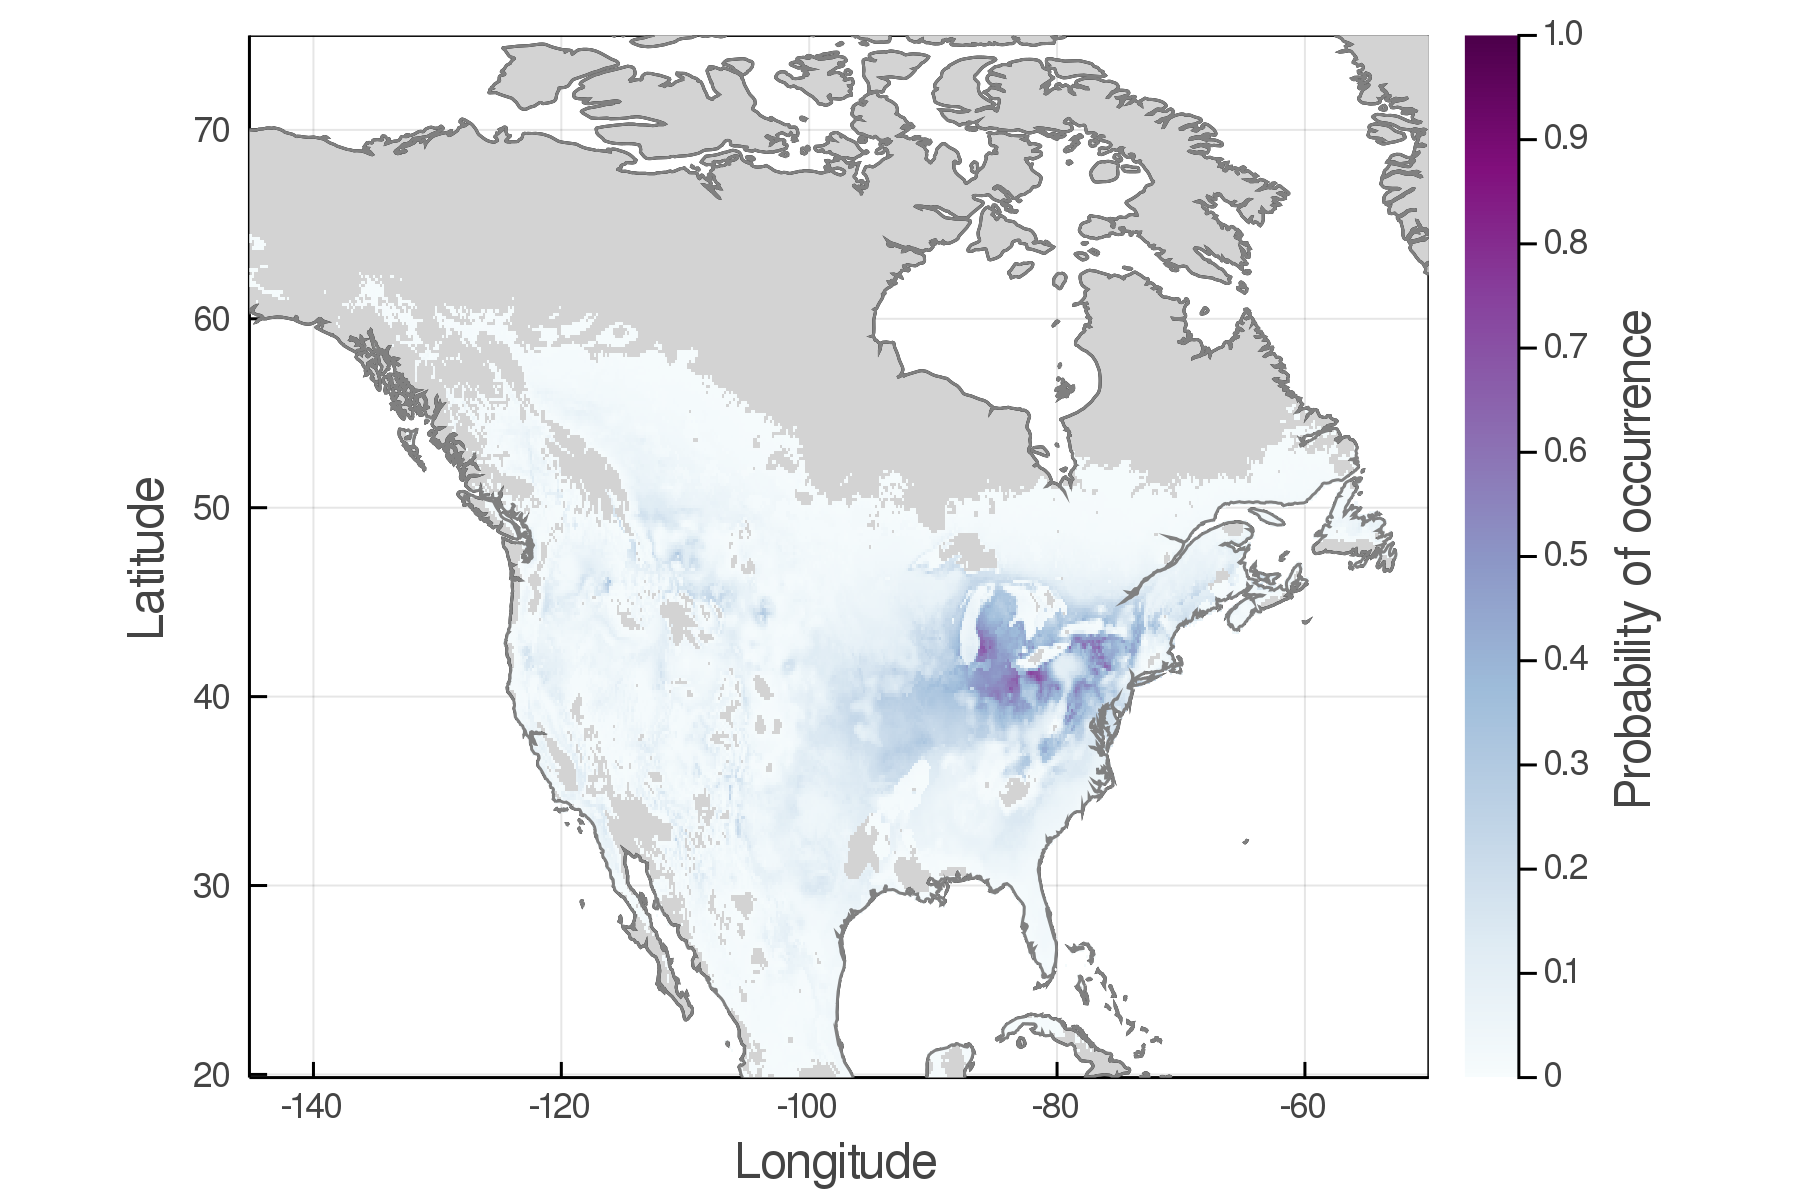
\includegraphics[scale=0.17]{fig/01_sdm_singlesp-threshold.png}
  \end{figure}
\end{frame}

\begin{frame}
  \frametitle{Single species example - SDM without threshold}
  \begin{figure}
    \centering
    \hspace*{-0cm}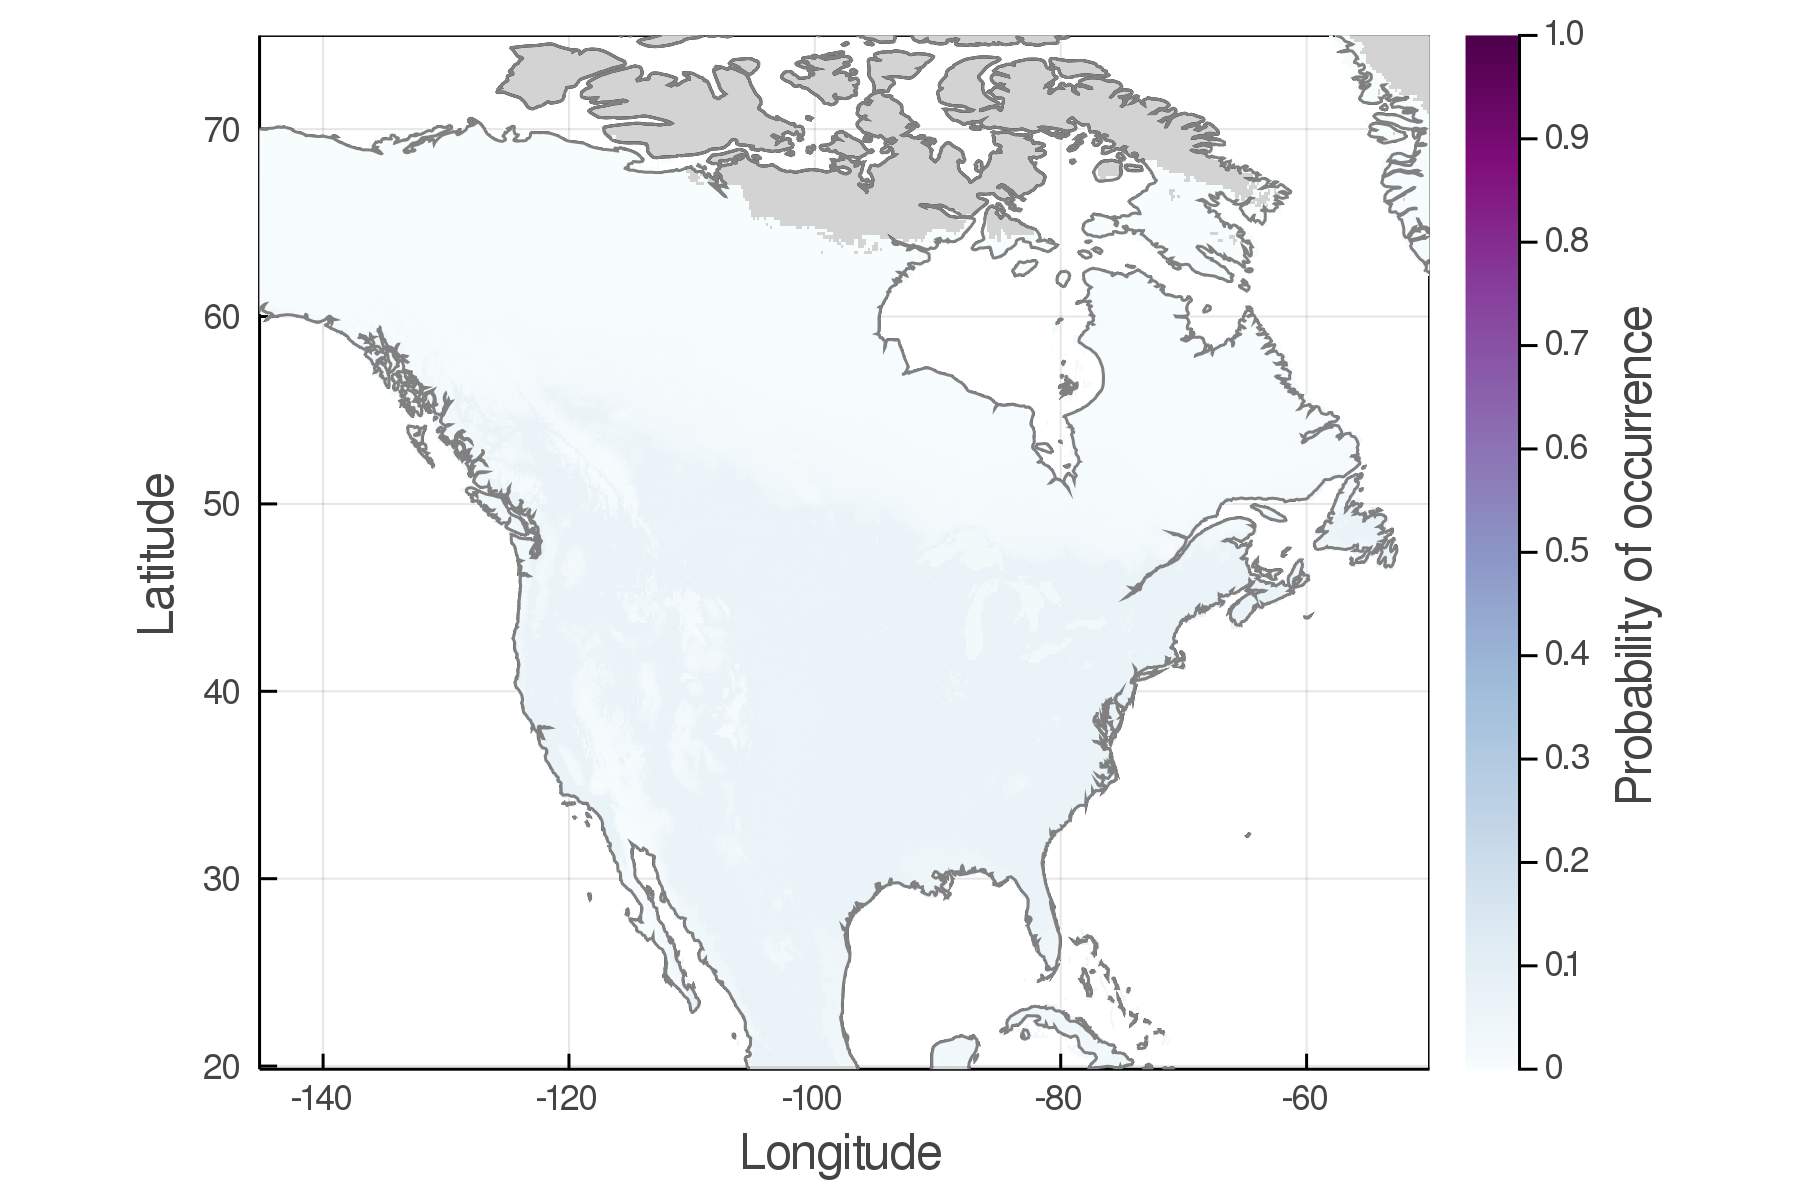
\includegraphics[scale=0.17]{fig/01_sdm_singlesp.png}
  \end{figure}
\end{frame}

\begin{frame}
  \frametitle{LCBD - Raw data (with Hellinger transformation)}
  \begin{figure}
    \centering
    \hspace*{-0cm}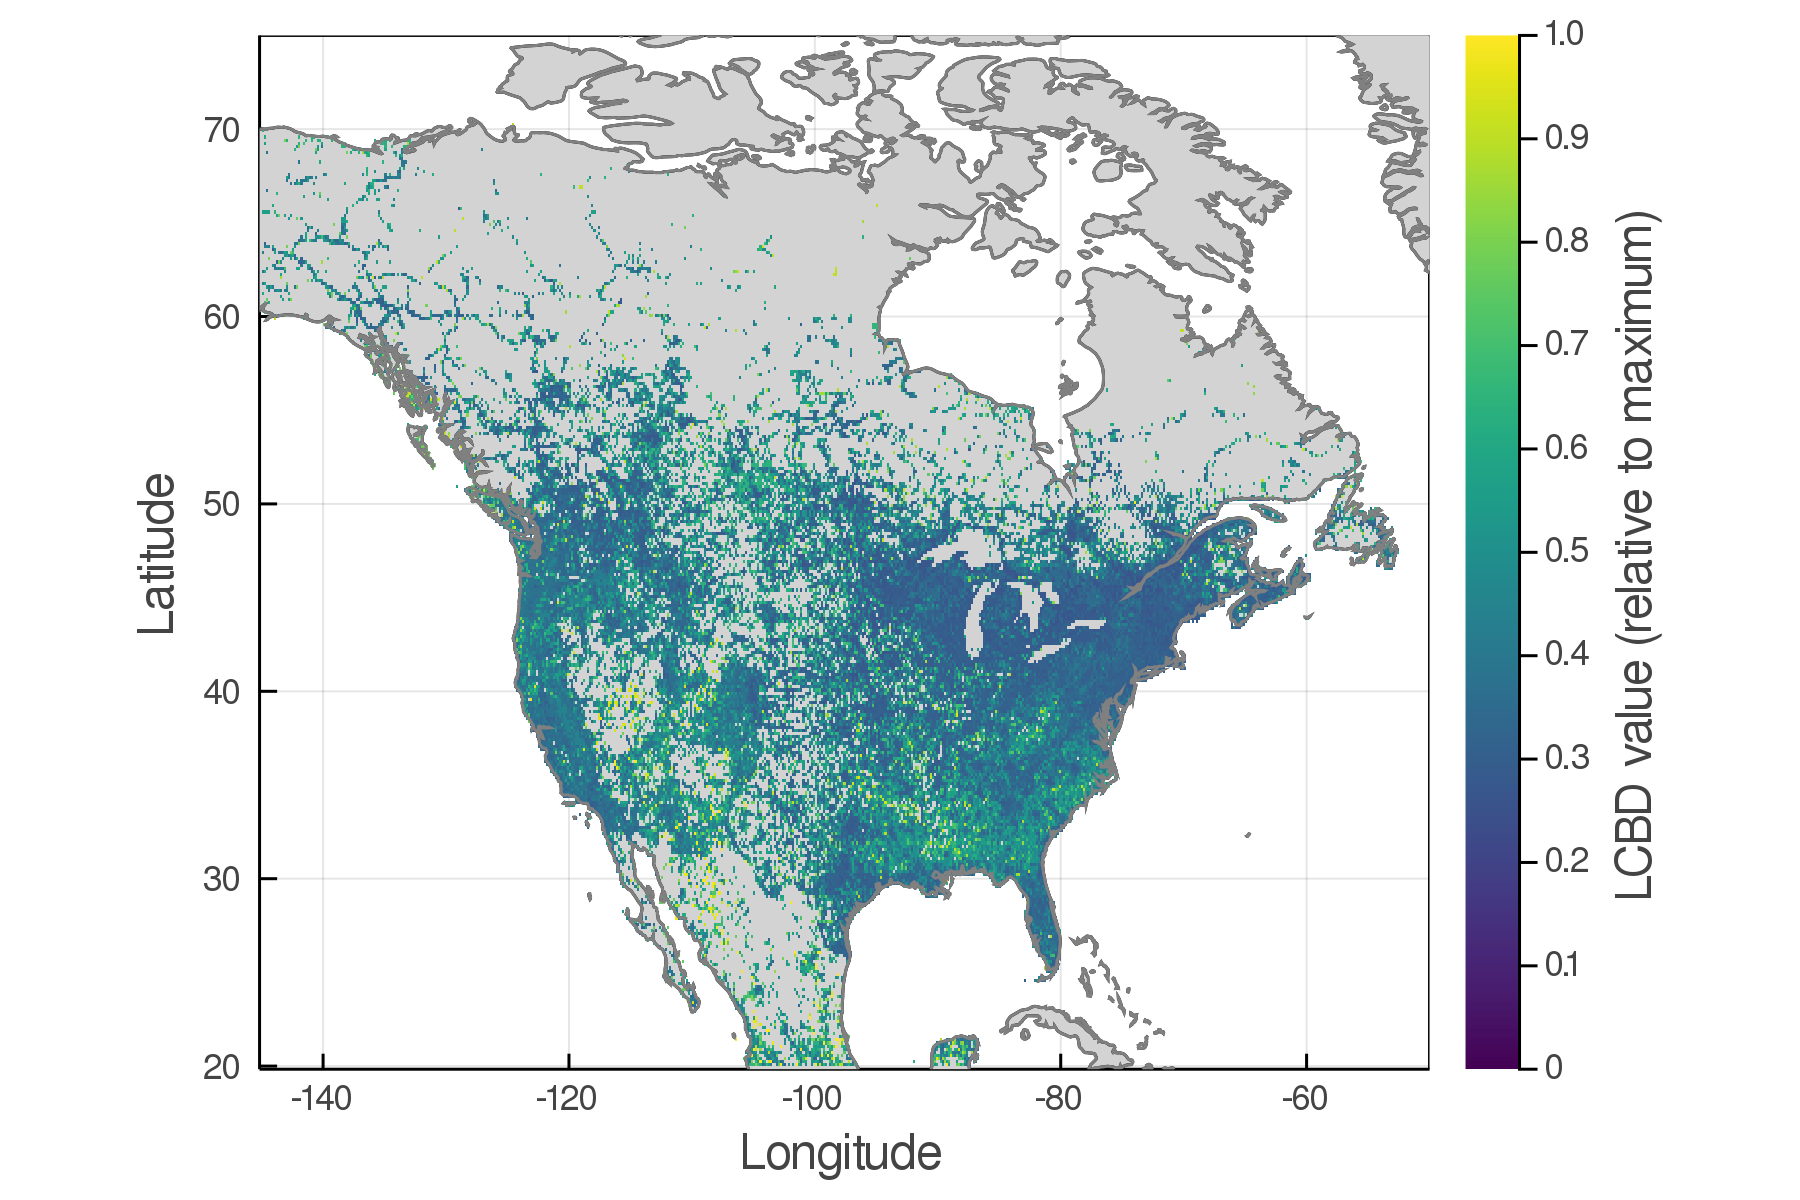
\includegraphics[scale=0.17]{fig/05_raw_lcbd-transf.png}
    \caption{LCBD values relative to maximum value based on the raw data after Hellinger transformation}
  \end{figure}
\end{frame}

\end{document}
